%&preformat-present

\newif\ifpresentation % Условие, проверяющее, что документ --- презентация
\presentationtrue
\documentclass[10pt, xcolor={dvipsnames, table, hyperref}]{beamer}

%%% Добавление поясняющих записей (notes) к презентации %%%
\makeatletter
\@ifundefined{c@presnotes}{
    \newcounter{presnotes}
    \setcounter{presnotes}{0}       % 0 --- выкл;
                                    % 1 --- вкл, записи на отдельном слайде;
                                    % 2 --- вкл, записи на основном слайде;
}{}
\makeatother

%%% Положение поясняющих записей (notes) при значении presnotes=2 %%%
\newcommand{\presposition}{left}  % возможные значения: left, right, top, bottom

%%% Добавление логотипа из файла images/logo на первом слайде %%%
\makeatletter
\@ifundefined{c@logotitle}{
    \newcounter{logotitle}
    \setcounter{logotitle}{1}       % 0 --- выкл;
                                    % 1 --- вкл
}{}
\makeatother

%%% Добавление логотипа из файла images/logo на слайдах (кроме первого и последнего) %%%
\makeatletter
\@ifundefined{c@logoother}{
    \newcounter{logoother}
    \setcounter{logoother}{0}       % 0 --- выкл;
                                    % 1 --- вкл
}{}
\makeatother
\usepackage{array,graphicx,caption}               % Общие настройки шаблона
%%% Проверка используемого TeX-движка %%%
\RequirePackage{ifxetex, ifluatex}
\newif\ifxetexorluatex   % определяем новый условный оператор (http://tex.stackexchange.com/a/47579)
\ifxetex
    \xetexorluatextrue
\else
    \ifluatex
        \xetexorluatextrue
    \else
        \xetexorluatexfalse
    \fi
\fi

\newif\ifsynopsis           % Условие, проверяющее, что документ --- автореферат

\RequirePackage{etoolbox}[2015/08/02]               % Для продвинутой проверки разных условий
\providebool{presentation}

%%% Поля и разметка страницы %%%
\usepackage{pdflscape}                              % Для включения альбомных страниц
\usepackage{geometry}                               % Для последующего задания полей

%%% Математические пакеты %%%
\usepackage{amsthm,amsmath,amscd}   % Математические дополнения от AMS
\usepackage{amsfonts,amssymb}       % Математические дополнения от AMS
\usepackage{mathtools}              % Добавляет окружение multlined
\usepackage{xfrac}                  % Красивые дроби
\usepackage[
    locale = DE,
    list-separator       = {;\,},
    list-final-separator = {;\,},
    list-pair-separator  = {;\,},
    range-phrase={\text{\ensuremath{-}}},
    % quotient-mode        = fraction, % красивые дроби могут не соответствовать ГОСТ
    fraction-function    = \sfrac,
    separate-uncertainty,
    ]{siunitx}                      % Размерности SI
\sisetup{inter-unit-product = \ensuremath{{}\cdot{}}}

% Кириллица в нумерации subequations
% Для правильной работы требуется выполнение сразу после загрузки пакетов
\patchcmd{\subequations}{\def\theequation{\theparentequation\alph{equation}}}
{\def\theequation{\theparentequation\asbuk{equation}}}
{\typeout{subequations patched}}{\typeout{subequations not patched}}

%%%% Установки для размера шрифта 14 pt %%%%
%% Формирование переменных и констант для сравнения (один раз для всех подключаемых файлов)%%
%% должно располагаться до вызова пакета fontspec или polyglossia, потому что они сбивают его работу
\newlength{\curtextsize}
\newlength{\bigtextsize}
\setlength{\bigtextsize}{13.9pt}

\makeatletter
%\show\f@size                                       % неплохо для отслеживания, но вызывает стопорение процесса, если документ компилируется без команды  -interaction=nonstopmode
\setlength{\curtextsize}{\f@size pt}
\makeatother

%%% Кодировки и шрифты %%%
\ifxetexorluatex
    \usepackage{polyglossia}[2014/05/21]            % Поддержка многоязычности (fontspec подгружается автоматически)
\else
   %%% Решение проблемы копирования текста в буфер кракозябрами
    \ifnumequal{\value{usealtfont}}{0}{}{
        \input glyphtounicode.tex
        \input glyphtounicode-cmr.tex %from pdfx package
        \pdfgentounicode=1
    }
    \usepackage{cmap}                               % Улучшенный поиск русских слов в полученном pdf-файле
    \ifnumequal{\value{usealtfont}}{2}{}{
        \defaulthyphenchar=127                      % Если стоит до fontenc, то переносы не впишутся в выделяемый текст при копировании его в буфер обмена
    }
    \usepackage{textcomp}
    \usepackage[T1,T2A]{fontenc}                    % Поддержка русских букв
    \ifnumequal{\value{usealtfont}}{1}{% Используется pscyr, при наличии
        \IfFileExists{pscyr.sty}{\usepackage{pscyr}}{}  % Подключение pscyr
    }{}
    \usepackage[utf8]{inputenc}[2014/04/30]         % Кодировка utf8
    \usepackage[english, russian]{babel}[2014/03/24]% Языки: русский, английский
    \ifnumequal{\value{usealtfont}}{2}{
        % http://dxdy.ru/post1238763.html#p1238763
        \usepackage[scaled=0.960]{XCharter}[2017/12/19] % Подключение русифицированных шрифтов XCharter
        \usepackage[charter, vvarbb, scaled=1.048]{newtxmath}[2017/12/14]
        \ifpresentation
        \else
            \setDisplayskipStretch{-0.078}
        \fi
    }{}
\fi

%%% Оформление абзацев %%%
\usepackage{indentfirst}                            % Красная строка

%%% Цвета %%%
\ifpresentation
\else
    \usepackage[dvipsnames, table, hyperref]{xcolor} % Совместимо с tikz
\fi

%%% Таблицы %%%
\usepackage{longtable,ltcaption}                    % Длинные таблицы
\usepackage{multirow,makecell}                      % Улучшенное форматирование таблиц

%%% Общее форматирование
\usepackage{soulutf8}                               % Поддержка переносоустойчивых подчёркиваний и зачёркиваний
\usepackage{icomma}                                 % Запятая в десятичных дробях

%%% Оптимизация расстановки переносов и длины последней строки абзаца
\IfFileExists{impnattypo.sty}{% проверка установленности пакета impnattypo
    \ifluatex
        \ifnumequal{\value{draft}}{1}{% Черновик
            \usepackage[hyphenation, lastparline, nosingleletter, homeoarchy,
            rivers, draft]{impnattypo}
        }{% Чистовик
            \usepackage[hyphenation, lastparline, nosingleletter]{impnattypo}
        }
    \else
        \usepackage[hyphenation, lastparline]{impnattypo}
    \fi
}{}

%%% Гиперссылки %%%
\usepackage{hyperref}[2012/11/06]

%%% Изображения %%%
\usepackage{graphicx}[2014/04/25]                   % Подключаем пакет работы с графикой

%%% Счётчики %%%
\usepackage[figure,table]{totalcount}               % Счётчик рисунков и таблиц
\usepackage{totcount}                               % Пакет создания счётчиков на основе последнего номера подсчитываемого элемента (может требовать дважды компилировать документ)
\usepackage{totpages}                               % Счётчик страниц, совместимый с hyperref (ссылается на номер последней страницы). Желательно ставить последним пакетом в преамбуле

%%% Продвинутое управление групповыми ссылками (пока только формулами) %%%
\ifpresentation
\else
    \usepackage[russian]{cleveref} % cleveref имеет сложности со считыванием
    % языка из babel. Такое решение русификации вывода выбрано вместо
    % определения в documentclass из опасности что-то лишнее передать во все
    % остальные пакеты, включая библиографию.
    \creflabelformat{equation}{#2#1#3} % Формат по умолчанию ставил круглые
    % скобки вокруг каждого номера ссылки, теперь просто номера ссылок без
    % какого-либо дополнительного оформления
    \crefrangelabelformat{equation}{#3#1#4\cyrdash#5#2#6} % Интервалы в русском
    % языке принято делать через тире, если иное не оговорено

    % решение проблемы с "и" в \labelcref
    % https://tex.stackexchange.com/a/455124/104425
    \ifxetexorluatex
        \DeclareTextSymbol{\cyri}\UnicodeEncodingName{"0438} % и
    \fi

    % Добавление возможности использования пробелов в \labelcref
    % https://tex.stackexchange.com/a/340502/104425
    \usepackage{kvsetkeys}
    \makeatletter
    \let\org@@cref\@cref
    \renewcommand*{\@cref}[2]{%
        \edef\process@me{%
            \noexpand\org@@cref{#1}{\zap@space#2 \@empty}%
        }\process@me
    }
    \makeatother
\fi

\ifnumequal{\value{draft}}{1}{% Черновик
    \usepackage[firstpage]{draftwatermark}
    \SetWatermarkText{DRAFT}
    \SetWatermarkFontSize{14pt}
    \SetWatermarkScale{15}
    \SetWatermarkAngle{45}
}{}

%%% Исправление положения якорей подписей (под)рисунков %%%
% Без hypcap и патча, при клике по ссылке на подрисунок, просмотрщик pdf прыгает "к подписи" а не "к рисунку".
% Подробнее: https://github.com/AndreyAkinshin/Russian-Phd-LaTeX-Dissertation-Template/issues/238
% (!) Даже с патчем, если мешать в одной фиге разные типы подфиг (subbottom и subcaption) - ссылки всё равно будут работать неправильно  (см. https://www.overleaf.com/read/czmbmmtnqrrg ).
\ifpresentation
\else
    \usepackage[all]{hypcap}

    \makeatletter
    \ltx@ifclasslater{memoir}{2018/12/13}{
        % Предполагается, что в следующей версии класс будет исправлен
        \typeout{Assuming this version of memoir is free from the jumping-to-caption bug.}
    }{
        \RequirePackage{xpatch}

        \newcommand\mem@step@subcounter{\refstepcounter{sub\@captype}\@contkeep}

        \xpatchcmd{\@memsubbody}%
        {\refstepcounter{sub\@captype}\@contkeep}% search pattern
        {}% replacement
        {\typeout{@memsubbody is patched}}%
        {\typeout{@memsubbody is NOT patched}}%

        \xpatchcmd{\@memcontsubbody}%
        {\refstepcounter{sub\@captype}\@contkeep}% pattern
        {}% replacement
        {\typeout{@memcontsubbody is patched}}%
        {\typeout{@memcontsubbody is NOT patched}}%

        \xpatchcmd{\@memsubfloat}%
        {\vbox\bgroup}% search pattern
        {\vbox\bgroup\mem@step@subcounter}% replacement
        {\typeout{@memsubfloat patch is ok}}%
        {\typeout{@memsubfloat patch is NOT ok}}%

        \xpatchcmd{\subcaption}%
        {\refstepcounter{sub\@captype}}% search pattern
        {\H@refstepcounter{sub\@captype}}% replacement
        {\typeout{subcaption second patch is ok}}%
        {\typeout{subcaption second patch is NOT ok}}%
    }
    \makeatother
\fi

%%% Цитата, не приводимая в автореферате:
% возможно, актуальна только для biblatex
%\newcommand{\citeinsynopsis}[1]{\ifsynopsis\else ~\cite{#1} \fi}

%% Векторная графика

\usepackage{tikz}                   % Продвинутый пакет векторной графики
\usetikzlibrary{chains}             % Для примера tikz рисунка
\usetikzlibrary{shapes.geometric}   % Для примера tikz рисунка
\usetikzlibrary{shapes.symbols}     % Для примера tikz рисунка
\usetikzlibrary{arrows}             % Для примера tikz рисунка

%%Добавила
\usetikzlibrary{calc}
\usetikzlibrary{decorations.pathreplacing}
\usetikzlibrary{positioning}



% если текущий процесс запущен библиотекой tikz-external, то прекомпиляция должна быть включена
\ifdefined\tikzexternalrealjob
    \setcounter{imgprecompile}{1}
\fi

\ifnumequal{\value{imgprecompile}}{1}{% Только если у нас включена предкомпиляция
    \usetikzlibrary{external}   % подключение возможности предкомпиляции
    \tikzexternalize[prefix=images/cache/] % activate! % здесь можно указать отдельную папку для скомпилированных файлов
    \ifxetex
        \tikzset{external/up to date check={diff}}
    \fi
}{}
            % Пакеты общие для диссертации и автореферата
%%% Основные сведения %%%
\newcommand{\thesisAuthorLastName}{Васеева}
\newcommand{\thesisAuthorOtherNames}{Татьяна Валериевна}
\newcommand{\thesisAuthorInitials}{Т.\,В.}
\newcommand{\thesisAuthor}             % Диссертация, ФИО автора
{%
    \texorpdfstring{% \texorpdfstring takes two arguments and uses the first for (La)TeX and the second for pdf
        \thesisAuthorLastName~\thesisAuthorOtherNames% так будет отображаться на титульном листе или в тексте, где будет использоваться переменная
    }{%
        \thesisAuthorLastName, \thesisAuthorOtherNames% эта запись для свойств pdf-файла. В таком виде, если pdf будет обработан программами для сбора библиографических сведений, будет правильно представлена фамилия.
    }
}
\newcommand{\thesisAuthorShort}        % Диссертация, ФИО автора инициалами
{\thesisAuthorInitials~\thesisAuthorLastName}
%\newcommand{\thesisUdk}                % Диссертация, УДК
%{\todo{xxx.xxx}}
\newcommand{\thesisTitle}              % Диссертация, название
{\textsc{совершенствование математической модели многотонального сигнала и численных методов оценки параметров его гармоник}}
\newcommand{\thesisSpecialtyNumber}    % Диссертация, специальность, номер
{05.13.18}
\newcommand{\thesisSpecialtyTitle}     % Диссертация, специальность, название (название взято с сайта ВАК для примера)
{Математическое моделирование, численные методы и комплексы программ}
%% \newcommand{\thesisSpecialtyTwoNumber} % Диссертация, вторая специальность, номер
%% {\todo{XX.XX.XX}}
%% \newcommand{\thesisSpecialtyTwoTitle}  % Диссертация, вторая специальность, название
%% {\todo{Теория и~методика физического воспитания, спортивной тренировки,
%% оздоровительной и~адаптивной физической культуры}}
\newcommand{\thesisDegree}             % Диссертация, ученая степень
{кандидата технических наук}
\newcommand{\thesisDegreeShort}        % Диссертация, ученая степень, краткая запись
{канд. техн. наук}
\newcommand{\thesisCity}               % Диссертация, город написания диссертации
{Омск}
\newcommand{\thesisYear}               % Диссертация, год написания диссертации
{2020}
\newcommand{\thesisOrganization}       % Диссертация, организация
{Федеральное государственное бюджетное образовательное учреждение высшего
образования <<Омский государственный университет путей сообщения>> (ОмГУПС)}
\newcommand{\thesisOrganizationShort}  % Диссертация, краткое название организации для доклада
{\todo{НазУчДисРаб}}

\newcommand{\thesisInOrganization}     % Диссертация, организация в предложном падеже: Работа выполнена в ...
{<<федеральном государственном бюджетном образовательном учреждении высшего профессионального образования «Омский государственный университет путей сообщения (ОмГУПС (ОмИИТ)>>}

%% \newcommand{\supervisorDead}{}           % Рисовать рамку вокруг фамилии
\newcommand{\supervisorFio}              % Научный руководитель, ФИО
{Альтман Евгений Анатольевич}
\newcommand{\supervisorRegalia}          % Научный руководитель, регалии
{кандидат технических наук, доцент}
\newcommand{\supervisorFioShort}         % Научный руководитель, ФИО
{Е.\,А.~Альтман}
\newcommand{\supervisorRegaliaShort}     % Научный руководитель, регалии
{\todo{уч.~ст.,~уч.~зв.}}

%% \newcommand{\supervisorTwoDead}{}        % Рисовать рамку вокруг фамилии
%% \newcommand{\supervisorTwoFio}           % Второй научный руководитель, ФИО
%% {\todo{Фамилия Имя Отчество}}
%% \newcommand{\supervisorTwoRegalia}       % Второй научный руководитель, регалии
%% {\todo{уч. степень, уч. звание}}
%% \newcommand{\supervisorTwoFioShort}      % Второй научный руководитель, ФИО
%% {\todo{И.\,О.~Фамилия}}
%% \newcommand{\supervisorTwoRegaliaShort}  % Второй научный руководитель, регалии
%% {\todo{уч.~ст.,~уч.~зв.}}

\newcommand{\opponentOneFio}           % Оппонент 1, ФИО
{\todo{Фамилия Имя Отчество}}
\newcommand{\opponentOneRegalia}       % Оппонент 1, регалии
{\todo{доктор физико-математических наук, профессор}}
\newcommand{\opponentOneJobPlace}      % Оппонент 1, место работы
{\todo{Не очень длинное название для места работы}}
\newcommand{\opponentOneJobPost}       % Оппонент 1, должность
{\todo{старший научный сотрудник}}

\newcommand{\opponentTwoFio}           % Оппонент 2, ФИО
{\todo{Фамилия Имя Отчество}}
\newcommand{\opponentTwoRegalia}       % Оппонент 2, регалии
{\todo{кандидат физико-математических наук}}
\newcommand{\opponentTwoJobPlace}      % Оппонент 2, место работы
{\todo{Основное место работы c длинным длинным длинным длинным названием}}
\newcommand{\opponentTwoJobPost}       % Оппонент 2, должность
{\todo{старший научный сотрудник}}

%% \newcommand{\opponentThreeFio}         % Оппонент 3, ФИО
%% {\todo{Фамилия Имя Отчество}}
%% \newcommand{\opponentThreeRegalia}     % Оппонент 3, регалии
%% {\todo{кандидат физико-математических наук}}
%% \newcommand{\opponentThreeJobPlace}    % Оппонент 3, место работы
%% {\todo{Основное место работы c длинным длинным длинным длинным названием}}
%% \newcommand{\opponentThreeJobPost}     % Оппонент 3, должность
%% {\todo{старший научный сотрудник}}

\newcommand{\leadingOrganizationTitle} % Ведущая организация, дополнительные строки. Удалить, чтобы не отображать в автореферате
{\todo{Омский научно-исследовательский институт приборостроения (АО «ОНИИП»)}}

\newcommand{\defenseDate}              % Защита, дата
{\todo{18 декабря 2021~г.~в~15 часов}}
\newcommand{\defenseCouncilNumber}     % Защита, номер диссертационного совета
{\todo{Д\,212.178.15}}				   %05.13.18 – Математическое моделирование, численные методы и комплексы программ (технические науки).
\newcommand{\defenseCouncilTitle}      % Защита, учреждение диссертационного совета
{\todo{Омском государственном техническом университете}}
\newcommand{\defenseCouncilAddress}    % Защита, адрес учреждение диссертационного совета
{\todo{г.~Омск, проспект~Мира, 11}}
\newcommand{\defenseCouncilPhone}      % Телефон для справок
{\todo{+7~(3812)~65-64-92}}
\newcommand{\defenseCouncilmail}    
 {\todo{E-mail:~dissov\_omgtu@omgtu.ru}}                      %e-mail

\newcommand{\defenseSecretaryFio}      % Секретарь диссертационного совета, ФИО
{\todo{Варепо Лариса Григорьевна}}
\newcommand{\defenseSecretaryRegalia}  % Секретарь диссертационного совета, регалии
{\todo{доктор технических наук, доцент}}            % Для сокращений есть ГОСТы, например: ГОСТ Р 7.0.12-2011 + http://base.garant.ru/179724/#block_30000

\newcommand{\synopsisLibrary}          % Автореферат, название библиотеки
{\todo{Омского государственного технического университета}}
\newcommand{\synopsisDate}             % Автореферат, дата рассылки
{\todo{23 июля 2021 года}}

% To avoid conflict with beamer class use \providecommand
\providecommand{\keywords}%            % Ключевые слова для метаданных PDF диссертации и автореферата
{}
                % Основные сведения
%%% Кодировки и шрифты %%%
\ifxetexorluatex
    \setmainlanguage[babelshorthands=true]{russian}    % Язык по-умолчанию русский с поддержкой приятных команд пакета babel
    \setotherlanguage{english}                         % Дополнительный язык = английский (в американской вариации по-умолчанию)

    % Проверка существования шрифтов. Недоступна в pdflatex
    \ifnumequal{\value{fontfamily}}{1}{
        \IfFontExistsTF{Times New Roman}{}{\setcounter{fontfamily}{0}}
    }{}
    \ifnumequal{\value{fontfamily}}{2}{
        \IfFontExistsTF{LiberationSerif}{}{\setcounter{fontfamily}{0}}
    }{}

    \ifnumequal{\value{fontfamily}}{0}{                    % Семейство шрифтов CMU. Используется как fallback
        \setmonofont{CMU Typewriter Text}                  % моноширинный шрифт
        \newfontfamily\cyrillicfonttt{CMU Typewriter Text} % моноширинный шрифт для кириллицы
        \defaultfontfeatures{Ligatures=TeX}                % стандартные лигатуры TeX, замены нескольких дефисов на тире и т. п. Настройки моноширинного шрифта должны идти до этой строки, чтобы при врезках кода программ в коде не применялись лигатуры и замены дефисов
        \setmainfont{CMU Serif}                            % Шрифт с засечками
        \newfontfamily\cyrillicfont{CMU Serif}             % Шрифт с засечками для кириллицы
        \setsansfont{CMU Sans Serif}                       % Шрифт без засечек
        \newfontfamily\cyrillicfontsf{CMU Sans Serif}      % Шрифт без засечек для кириллицы
    }

    \ifnumequal{\value{fontfamily}}{1}{                    % Семейство MS шрифтов
        \setmonofont{Courier New}                          % моноширинный шрифт
        \newfontfamily\cyrillicfonttt{Courier New}         % моноширинный шрифт для кириллицы
        \defaultfontfeatures{Ligatures=TeX}                % стандартные лигатуры TeX, замены нескольких дефисов на тире и т. п. Настройки моноширинного шрифта должны идти до этой строки, чтобы при врезках кода программ в коде не применялись лигатуры и замены дефисов
        \setmainfont{Times New Roman}                      % Шрифт с засечками
        \newfontfamily\cyrillicfont{Times New Roman}       % Шрифт с засечками для кириллицы
        \setsansfont{Arial}                                % Шрифт без засечек
        \newfontfamily\cyrillicfontsf{Arial}               % Шрифт без засечек для кириллицы
    }

    \ifnumequal{\value{fontfamily}}{2}{                    % Семейство шрифтов Liberation (https://pagure.io/liberation-fonts)
        \setmonofont{LiberationMono}[Scale=0.87] % моноширинный шрифт
        \newfontfamily\cyrillicfonttt{LiberationMono}[     % моноширинный шрифт для кириллицы
            Scale=0.87]
        \defaultfontfeatures{Ligatures=TeX}                % стандартные лигатуры TeX, замены нескольких дефисов на тире и т. п. Настройки моноширинного шрифта должны идти до этой строки, чтобы при врезках кода программ в коде не применялись лигатуры и замены дефисов
        \setmainfont{LiberationSerif}                      % Шрифт с засечками
        \newfontfamily\cyrillicfont{LiberationSerif}       % Шрифт с засечками для кириллицы
        \setsansfont{LiberationSans}                       % Шрифт без засечек
        \newfontfamily\cyrillicfontsf{LiberationSans}      % Шрифт без засечек для кириллицы
    }

\else
    \ifnumequal{\value{usealtfont}}{1}{% Используется pscyr, при наличии
        \IfFileExists{pscyr.sty}{\renewcommand{\rmdefault}{ftm}}{}
    }{}
\fi







               % Определение шрифтов (частичное)

%%% Добавление поясняющих записей (notes) к презентации %%%
\makeatletter
\@ifundefined{c@presnotes}{
    \newcounter{presnotes}
    \setcounter{presnotes}{0}       % 0 --- выкл;
                                    % 1 --- вкл, записи на отдельном слайде;
                                    % 2 --- вкл, записи на основном слайде;
}{}
\makeatother

%%% Положение поясняющих записей (notes) при значении presnotes=2 %%%
\newcommand{\presposition}{left}  % возможные значения: left, right, top, bottom

%%% Добавление логотипа из файла images/logo на первом слайде %%%
\makeatletter
\@ifundefined{c@logotitle}{
    \newcounter{logotitle}
    \setcounter{logotitle}{1}       % 0 --- выкл;
                                    % 1 --- вкл
}{}
\makeatother

%%% Добавление логотипа из файла images/logo на слайдах (кроме первого и последнего) %%%
\makeatletter
\@ifundefined{c@logoother}{
    \newcounter{logoother}
    \setcounter{logoother}{0}       % 0 --- выкл;
                                    % 1 --- вкл
}{}
\makeatother
\usepackage{array,graphicx,caption}         % Настройки презентации
\input{Presentation/prespackages}  % Библиотеки презентации
% Общие стили оформления.
% Возможные варианты значений ищите в описании библиотеки beamer
\usecolortheme{whale}
%\usecolortheme{orchid}
%\usecolortheme{wolverine}
%\usecolortheme{lily}
%\usecolortheme{default}
%\usecolortheme{albatross}
%\usecolortheme{dolphin}
%\usecolortheme{sidebartab}
%\usecolortheme{beaver}
%\usecolortheme{crane}
%\usecolortheme{dove}
%\usecolortheme{beetle}


% Стиль презентации
%\usetheme[hideothersubsections]{Goettingen}
%\usetheme[hideothersubsections]{Boadilla}
%\usetheme{PaloAlto}
%\usetheme{default}
%\usetheme{AnnArbor}
%\usetheme{Antibes}
%\usetheme{Bergen}
%\usetheme{Berkeley}
%\usetheme{Berlin}
%\usetheme{Boadilla}
%\usetheme{CambridgeUS}
%\usetheme{Copenhagen}
%\usetheme{Darmstadt}
%\usetheme{Dresden}
%\usetheme{Frankfurt}
%\usetheme{Goettingen}
%\usetheme{Hannover}
%\usetheme{Ilmenau}
%\usetheme{JuanLesPins} 
%\usetheme{Luebeck}
%\usetheme{Madrid}
%\usetheme{Malmoe} 
%\usetheme{Marburg}
%\usetheme{Montpellier} 
\usetheme{Pittsburgh}
%\usetheme{Rochester}
%\usetheme{Singapore}
%\usetheme{Szeged}

%\usetheme{Warsaw}

% \usetheme[secheader]{Boadilla}
% \usecolortheme{seahorse}

% выключение кнопок навигации
\beamertemplatenavigationsymbolsempty

% Размеры шрифтов
\setbeamerfont{title}{size=\large}
\setbeamerfont{subtitle}{size=\small}
\setbeamerfont{author}{size=\normalsize}
\setbeamerfont{institute}{size=\small}
\setbeamerfont{date}{size=\normalsize}
\setbeamerfont{bibliography item}{size=\small}
\setbeamerfont{bibliography entry author}{size=\small}
\setbeamerfont{bibliography entry title}{size=\small}
\setbeamerfont{bibliography entry location}{size=\small}
\setbeamerfont{bibliography entry note}{size=\small}
%\setbeamerfont{footline}{size=\bf\Large}
\setbeamerfont{footline}{size=\bf\small}

% Аналогично можно настроить и другие размеры.
% Названия классов элементов можно найти здесь
% http://www.cpt.univ-mrs.fr/~masson/latex/Beamer-appearance-cheat-sheet.pdf

% Цвет элементов
\setbeamercolor{footline}{fg=blue}
%\setbeamercolor{footline}{fg=black}
\setbeamercolor{bibliography item}{fg=black}
\setbeamercolor{bibliography entry author}{fg=black}
\setbeamercolor{bibliography entry title}{fg=black}
\setbeamercolor{bibliography entry location}{fg=black}
\setbeamercolor{bibliography entry note}{fg=black}
% Аналогично можно настроить и другие цвета.
% Названия классов элементов можно найти здесь
% http://www.cpt.univ-mrs.fr/~masson/latex/Beamer-appearance-cheat-sheet.pdf

% Убрать иконки перед списком литературы
% https://tex.stackexchange.com/a/124271/104425
\setbeamertemplate{bibliography item}{}

% Использовать шрифт с засечками для формул
% https://tex.stackexchange.com/a/34267/104425
\usefonttheme[onlymath]{serif}

% https://tex.stackexchange.com/a/291545/104425
\makeatletter
\def\beamer@framenotesbegin{% at beginning of slide
    \usebeamercolor[fg]{normal text}
    \gdef\beamer@noteitems{}%
    \gdef\beamer@notes{}%
}
\makeatother

% footer презентации
\setbeamertemplate{footline}{
    \leavevmode%
    \hbox{%
        \begin{beamercolorbox}[wd=.333333\paperwidth,ht=2.25ex,dp=2ex,center]{}%
            % И. О. Фамилия, Организация кратко
            \thesisAuthorShort%, \thesisOrganizationShort
        \end{beamercolorbox}%
        \begin{beamercolorbox}[wd=.333333\paperwidth,ht=2.25ex,dp=2ex,center]{}%
            % Город, 20XX
            \thesisCity, \thesisYear
        \end{beamercolorbox}%
        \begin{beamercolorbox}[wd=.333333\paperwidth,ht=2.25ex,dp=2ex,right]{}%
            %Стр.
            {\LARGE \insertframenumber{}\hspace*{2ex}} % из \inserttotalframenumber \hspace*{2ex}
        \end{beamercolorbox}}%
    \vskip0pt%
}

% вывод на экран заметок к презентации
\ifnumequal{\value{presnotes}}{0}{}{
    \setbeameroption{show notes}
    \ifnumequal{\value{presnotes}}{2}{
        \setbeameroption{show notes on second screen=\presposition}
    }{}
}
        % Стили презентации
\setbeamertemplate{title page}
{
    \ifnumequal{\value{logotitle}}{1}{
        \IfFileExists{images/omgups.png}{
            \begin{minipage}[c]{0.15\textwidth}
                \begin{flushleft}
                    \usebeamercolor[fg]{titlegraphic}\inserttitlegraphic
                \end{flushleft}
            \end{minipage}%
            \hfill
            \begin{minipage}[c]{0.8\linewidth}
                \centering
                \usebeamerfont{institute}\insertinstitute\par
            \end{minipage}
        }{
            \centering
            \usebeamerfont{institute}\insertinstitute\par
        }
    }{
        \centering
        \usebeamerfont{institute}\insertinstitute\par
    }
    \centering
    \vfill
    \usebeamerfont{subtitle}\insertsubtitle\par
    \bigskip
    \usebeamerfont{title}\inserttitle\par
    \vfill
    \usebeamerfont{author}\insertauthor\par
    \vfill
    \usebeamerfont{date}\insertdate\par
}

%\title{\small{Название презентации}}
\title{\thesisTitle}
\author{%
    \texorpdfstring{%
        \begin{flushleft}
        	\emph{Выступающий:}~\thesisAuthorShort\\%
        \emph{Руководитель:}~\supervisorRegaliaShort~\supervisorFioShort\\%
        \end{flushleft}
         }{\thesisAuthor}%
}
\date{\texorpdfstring{\thesisCity, \thesisYear}{}}
\institute{\texorpdfstring{\thesisOrganization}{}}
\IfFileExists{images/omgups.png}{
    \titlegraphic{
\includegraphics[width=\textwidth]{images/omgups.png}}
    \ifnumequal{\value{logoother}}{1}{
        \logo{
\includegraphics[width=0.15\textwidth]{images/omgups.png}}
    }{}
}{}
\subtitle{Представление на соискание учёной степени \thesisDegree\ по специальности \thesisSpecialtyNumber\ \thesisSpecialtyTitle}
         % Настройки заглавной странице

%%% Библиография. Выбор движка для реализации %%%
\ifnumequal{\value{bibliosel}}{0}{%
    \input{biblio/predefined}   % Встроенная реализация с загрузкой файла через движок bibtex8
}{
    \input{biblio/biblatex}     % Реализация пакетом biblatex через движок biber
}

% Вывести информацию о версиях используемых библиотек в лог сборки
\listfiles


\begin{document}
\begin{frame}[noframenumbering,plain]
    \setcounter{framenumber}{1}
    \maketitle
\end{frame}      % Первые слайды презентации
\captionsetup[figure]{labelformat=simple, labelsep=period}
\section{Общие положения}

\subsection{Цель, объект и предмет исследования}
\begin{frame}{Цель, объект и предмет исследования}
	\textbf{Целью} работы является совершенствование методов оценки параметров гармоник многотонального сигнала. \vspace{1em}

	\textbf{Объектом} исследования являются методы оценки параметров гармоник в силовых электрических сетях. \vspace{1em}
	
	\textbf{Предметом} исследования является точность и быстродействие численных методов оценки параметров гармоник.	
\end{frame}

\subsection{Задачи исследования}
\begin{frame}{Задачи исследования}
	\begin{enumerate}
		\item Анализ математических основ объекта исследования и формулировка математической модели многотонального сигнала.
		\item Изучение и экспериментальное исследование алгоритмов оценки параметров гармоник.
		\item Развитие математической модели многотональных сигналов в части расчета точности оценки амплитуды применительно к используемому при оценке параметров гармоник подходу, связанному с применением оконных функций.
		\item Разработка численных методов для оценки параметров гармоник, позволяющих достичь расчетной точности для амплитуды гармоники.
		\item Разработка алгоритмов для эффективного выполнения численных методов из предыдущей задачи.
		\item Разработка комплекса программ для анализа и доработки алгоритмов оценки параметров гармоник многотональных сигналов.
	\end{enumerate}
\end{frame}

\subsection{Научная новизна работы}
\begin{frame}{Научная новизна работы}
	\begin{enumerate}
		\item Дополнена математическая модель спектра многотонального сигнала  полученными и экспериментально проверенными формулами для нахождения границы Крамера-Рао при оценке амплитуды гармоники для взвешенного оконной функцией сигнала.
		\item Предложен численный метод нахождения оптимальной несмещенной оценки амплитуды гармоники на основе корреляционного анализа, а также предложена его быстрая реализация на основе алгоритмов разряженного БПФ.
		\item Реализован комплекс программ для экспериментальной проверки полученных в работе формул и анализа алгоритмов оценки параметров гармоник многотональных сигналов.
	\end{enumerate}	
\end{frame}

\subsection{Практическая значимость работы}
\begin{frame}{Практическая значимость работы}
	\begin{enumerate}
		\item Выведена формула для нахождения границы Крамера-Рао при применении оконной функции, которая позволяет повысить эффективность научных исследований различных алгоритмов обработки сигналов с применением оконных функций, заменив моделирование алгоритма с применением различных окон расчетом по предложенной формуле.
		\item Предложенный численный метод, вместе с его быстрой реализацией, позволяют повысить точность и достоверность результатов измерительных приборов для электрических сетей.
		\item Разработанный комплекс программ позволяет проводить научные исследования в области цифровой обработки сигналов и используется в учебном процессе.
	\end{enumerate}
\end{frame}

\section{Математическая модель многотонального сигнала}
\subsection{Ограничение ДПФ}
\begin{frame}{Ограничение ДПФ}
\begin{tabular}{m{0.5\linewidth}m{0.5\linewidth}}
\textbf{Модель сигнала}:	
\begin{equation}
\label{eq:equation1}
s(t) = \displaystyle\sum_{k=0}^{N-1} A_k \cos \left({\frac{2 \pi}{T_s} f_{peak} t  + \varphi_k} \right)+ \eta(t)  
\end{equation}
\textbf{ДПФ}:		
\begin{equation}
\label{eq:equation3}
	\dot{X}(n)= \displaystyle\sum_{k=0}^{N-1} x(k) \cdot \exp\left( -j \cdot \frac{2 \pi n k}{N}\right)
\end{equation}  
%при $k=0,1, \cdots > N - 1$
&
\begin{figure}[ht]
%\centering
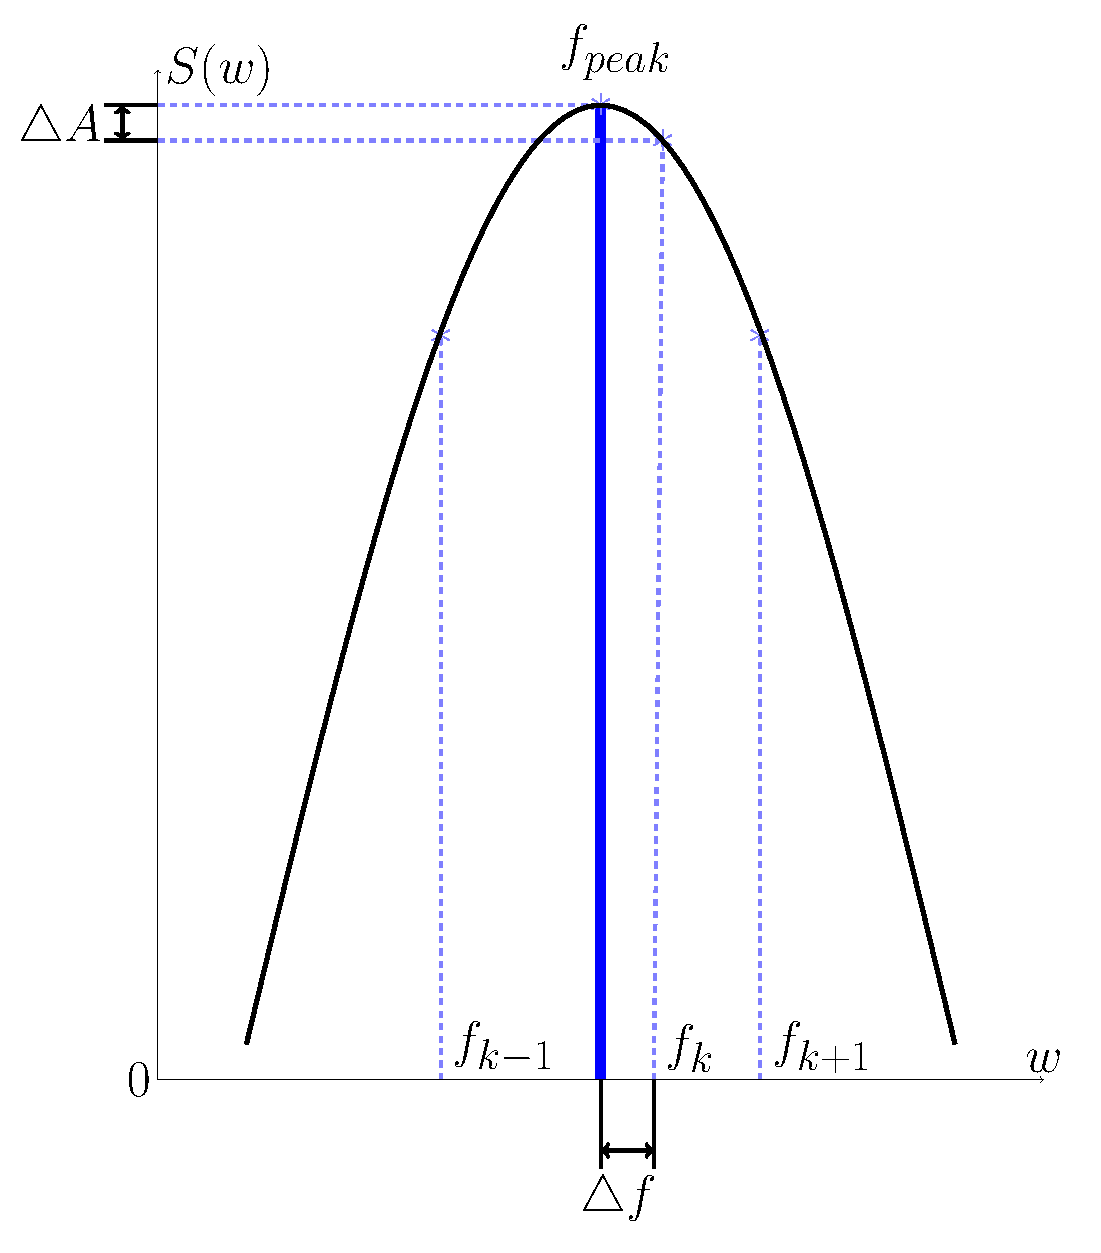
\includegraphics [scale=0.27] {Maximum_DFT.pdf}
\begin{flushright}
\caption{Случай несовпадения максимума ДПФ и максимума спектра гармоник.}	
\end{flushright}
\label{img:picture1}
\end{figure}
\end{tabular}
% E. Jacobsen and P. Kootsookos, "Fast, Accurate Frequency Estimators [DSP Tips & Tricks]," in IEEE Signal Processing Magazine, vol. 24, no. 3, pp. 123-125, May 2007, doi: 10.1109/MSP.2007.361611.
%Jacobsen E. On local interpolation of DFT outputs //Available online: http://www. ericjacobsen. org/FTinterp. pdf.[Accessed January 2013]. – 1994.
\end{frame}

\begin{frame}{Влияние оконной функции}
%	\textsc{Рисунок, показывающий, что происходит со спектром гармоники при наложении на него окна. Лучше в двух частях - с прямоугольным окном и окном Кайзера.}	
\begin{minipage}[t]{0.47\linewidth}
	\centering 
	\textbf{Прямоугольное окно}
	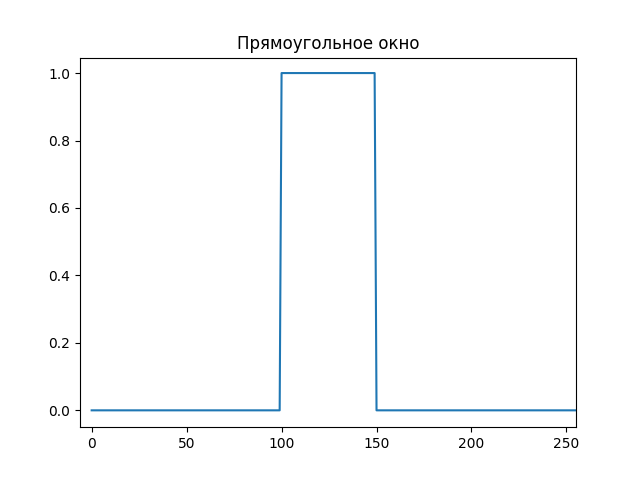
\includegraphics[width=.85\linewidth]{Прямоугольное окно040521.png}
	\textbf{Окно Кайзера}
	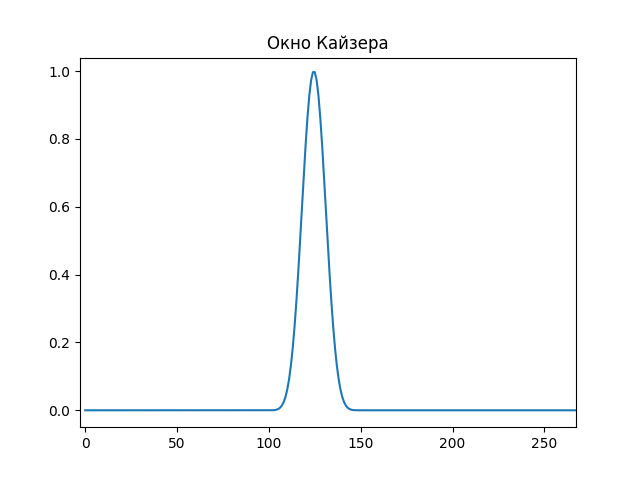
\includegraphics[width=.85\linewidth]{ОкноКазера040521.png}		
\end{minipage}
\hfill
\begin{minipage}[t]{0.47\linewidth}
	\centering 
	\textbf{Спектр с прям-ым окном}
	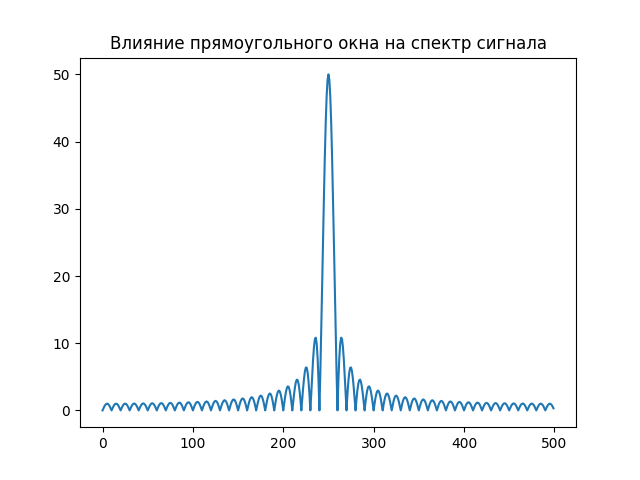
\includegraphics[width=.85\linewidth]{ПрямоугольныйСпект230421.png}
	\textbf{Спектр с окном Кайзера}
	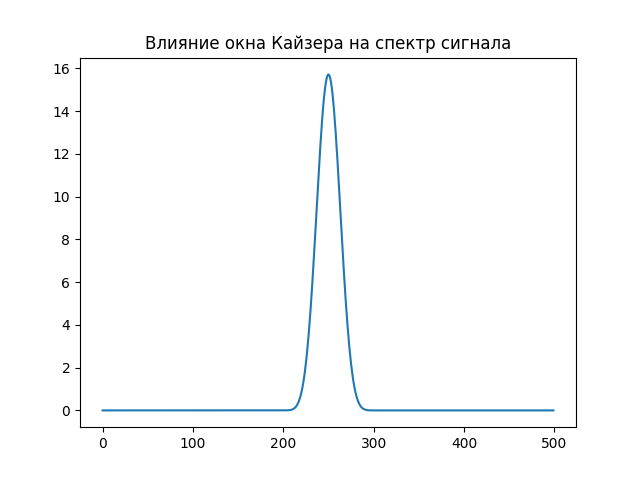
\includegraphics[width=.85\linewidth]{СпектрОкняКайзера230421.png}
\end{minipage}
\end{frame}

\begin{frame}{Методы интерполирования спектра}
\begin{tabular}{m{0.45\linewidth}m{0.45\linewidth}}
\small{
\begin{itemize}	
	\item Метод Якобсена;
	\item Два метода Квина;
	\item Два метода Маклеода;
	\item Метод Грэндка;
	\item Алгоритм параболической интерполяции;
	\item Алгоритм интерполяции Гаусса;
	\item Алгоритм, рекомендованный в ГОСТ 30804.4.7-2003;
	\item Метод корреляционных функций;
	\item Модернизированный метод корреляционных функций.				
\end{itemize}}
&	
%\textbf{Разность между дискретными гармониками:}
\begin{equation}
	\label{eq:equation2}
	\bigtriangleup f = \frac{(|X_{k+1}|-|X_{k-1}|)}{(4|X_{k}|-2|X_{k-1}|-2|X_{k+1}|)}
\end{equation}

\begin{equation}
	\label{eq:equation7}
	f_{peak} = f_k + \bigtriangleup f
\end{equation}
\begin{equation}
	\label{eq:equation8}
	f_{tone} = f_{peak} \cdot \frac{f_s}{N}
\end{equation}
%\begin{equation}
%	\label{eq:equation4}
%	u(f_k-1) = a \cdot (f_k-1-\bigtriangleup f)^2 + b
%\end{equation}
%\begin{equation}
%	\label{eq:equation5}
%	u(f_k) = a \cdot (f_k-\bigtriangleup f)^2+b,
%\end{equation}
%\begin{equation}
%	\label{eq:equation6}
%	u(f_k+1) = a\cdot (f_k+1-\bigtriangleup f)^2 +b
%\end{equation}
\end{tabular}
\end{frame}

\begin{frame}{Методы экстраполирования сигнала}
	\begin{minipage}[t]{0.45\linewidth}
		\centering 
		\textbf{Сигнал (частота=5.2)}
		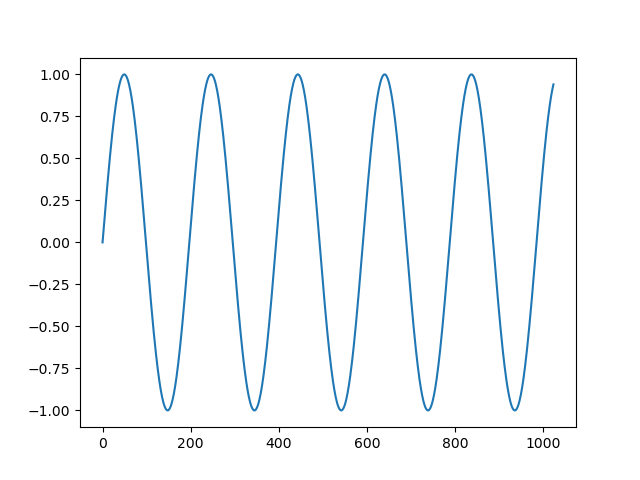
\includegraphics[width=.85\linewidth]{signal}
		\textbf{Экстраполированный сигнал }
		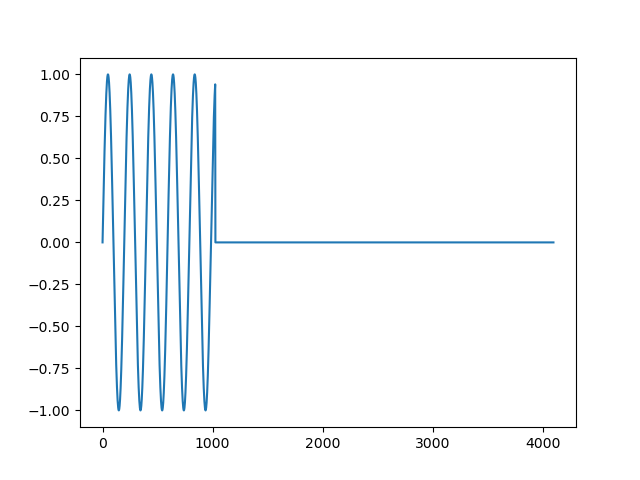
\includegraphics[width=.85\linewidth]{interpolated_signal}		
	\end{minipage}
	\hfill
	\begin{minipage}[t]{0.45\linewidth}
		\centering 
		\textbf{Спектр}
		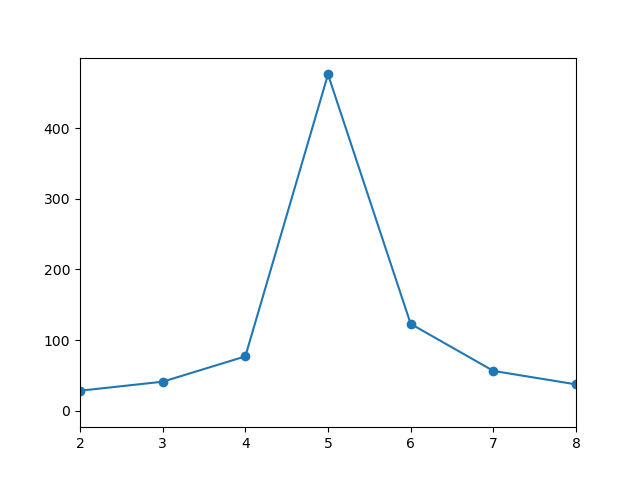
\includegraphics[width=.85\linewidth]{spectrum}
		\textbf{Спектр экстр. сигнала}
		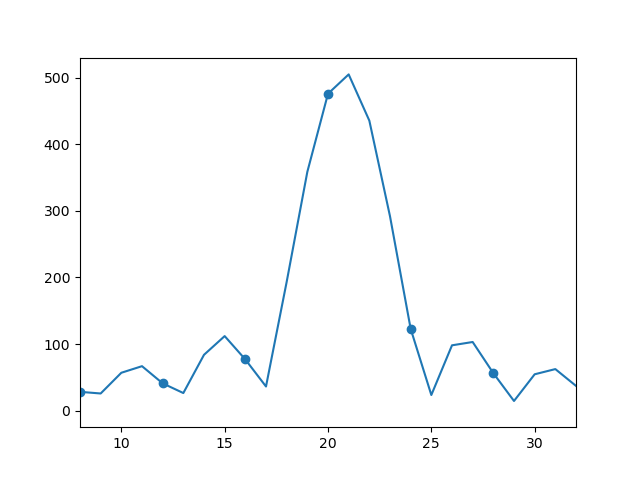
\includegraphics[width=.85\linewidth]{spectrum_of_interpolated_signal}
	\end{minipage}
\end{frame}

\subsection{Граница Крамера-Рао}
\begin{frame}{Общая формула границы Крамера-Рао}
%Теоретическая точность определения амплитуды гармоник	
\begin{tabular}{m{0.45\linewidth}m{0.45\linewidth}}
\textbf{Граница Крамера-Рао:}
\begin{equation}
\label{eq:equation13}
var(\theta)\geq \frac{1}{I(\theta)}
\end{equation}
$\theta$ – оцениваемый параметр;
		
$var(\theta)$ – дисперсия (variance) несмещенной оценки параметра.

\textbf{Информация Фишера:}
\begin{equation}
	\label{eq:equation14}
	I(\theta) = -E \left[\frac{\delta^2 ln p(x;\theta)}{\delta\theta^2}\right]
\end{equation}
где $E$ – среднее значение;

$p(x;\theta)$ – функция правдоподобия.
&
\textbf{Общая оценка границы Крамера-Рао для сигналов в белом Гауссовом шуме:}
\begin{equation}
	\label{eq:equation14}
x[n] = A + s[n;\theta] + w[n], n=0,1,...,N-1	
\end{equation}
$x[n]$ -- среднее значение;

$A$ и $\theta$  -- оцениваемые параметры;

$w[n]$ -- белый шум Гаусса;

$s[n;\theta]$ -- детерминированный сигнал.
\begin{equation}
\label{eq:equation14}
var(\hat{\theta}) \geq \frac{\sigma^2}{\displaystyle\sum_{n=0}^{N-1} \left(\frac{\partial s [n; \theta]}{\partial\theta}\right)^2} 
\end{equation}
\end{tabular}
\end{frame}

\begin{frame}{Неравенство Крамера-Рао для амплитуды, частоты и фазы гармоник}
\textbf{Матрица Фишера:}
\begin{equation}
\label{eq:equation15}
I(\theta) = \frac{1}{\sigma^2}
\begin{bmatrix}
	\frac{N}{2} & 0 & 0 \\
	0 & 2A^2 \pi^2 \displaystyle\sum_{n=0}^{N-1} n^2 & A^2 \pi \displaystyle\sum_{n=0}^{N-1} n \\
	0 & A^2 \pi \displaystyle\sum_{n=0}^{N-1} n & \dfrac{NA^2}{2}
\end{bmatrix}
\end{equation}
\begin{equation}
\label{eq:equation16}
var(\hat{A})\geq \frac{2  \sigma^2}{N} 
\end{equation}
\begin{equation}
\label{eq:equation17}
var(\hat{f_0})\geq \frac{12}{(2\pi)^2 \eta  N(N^2 - 1)}  
\end{equation}
%(3.41), C.34
\begin{equation}
\label{eq:equation18}
var(\hat{\varphi})\geq \frac{2(2N-1)}{\eta N(N+1)}  
\end{equation}
\end{frame}

\begin{frame}{Нахождение дисперсии результата оценки амплитуды}
\begin{tabular}{m{0.45\linewidth}m{0.45\linewidth}}
\textbf{Изменение дисперсии шума:}
\begin{equation}
\label{eq:equation19}
w g N_i = w_i \cdot w g N_i
\end{equation}
${\sigma^2}' = (w_i \cdot w g N_i - 0)^2=$
\begin{equation}
\label{eq:equation19}
(w_i \cdot w g N_i)^2 =\frac{\displaystyle\sum_{i=1}^{N-1} w_i^2}{N} \cdot \sigma^2
\end{equation}
\textbf{При изменении оцениваемой величины $\alpha=g(\theta)$ дисперсия изменяется:}

&
\begin{equation}
	\label{eq:equation19}
	var (\alpha) = \frac{ \left({\frac{\partial^2 g}{\partial \theta}}\right)^2}{-E \left(\frac{\partial ^2 \ln P(x; \theta)}{\partial \theta^2} \right) }
\end{equation}
\textbf{В нашем случае:}
\begin{equation}
\label{eq:equation19}
A'= \frac{A}{w_0}
\end{equation}
\textbf{Получаем:}
\begin{equation}
	\label{eq:equation19}
	var(A)= \frac{2\sigma^2}{N}\cdot \frac{N}{\displaystyle\sum_{i=1}^{N-1} w_i^2}
\end{equation}
\end{tabular}
\end{frame}


\begin{frame}{Математическая модель для оценки точности нахождения амплитуды гармоники}
\begin{tabular}{m{0.45\linewidth}m{0.45\linewidth}}
\begin{equation}
	\label{eq:equation24}
	var(A)\geq \frac{2\sigma^2}{N} \frac{\sum_{n=0}^{N-1}w_n^2}{\left(\sum_{n=0}^{N-1} w_n \right)^2} 			  
\end{equation}
где $\sigma$ -- среднее квадратичное отклонение шума;

$n$ – номер отчета.

$N$ – число отсчетов в дискретном сигнале;
 
$x(n;\theta)$ – наблюдаемый сигнал;

$A$ – амплитуда гармоники.
&
\textbf{Введем обозначение коэффициент окна:} 
\begin{equation}
	\label{eq:equation25}
	F_{win}=\frac{\sum_{n=0}^{N-1}w_n^2}{\left(\sum_{n=0}^{N-1} w_n\right)^2}
\end{equation}
Данный коэффициент показывает, во сколько ухудшится оценка амплитуды гармоники при использовании окна $w$.
\end{tabular}
\end{frame}
\note{\cite{altman2020boundary}}


\begin{frame}{Практическая точность методов}
\begin{tabular}{m{0.45\linewidth}m{0.45\linewidth}}
\begin{figure}[ht]
	\centering
	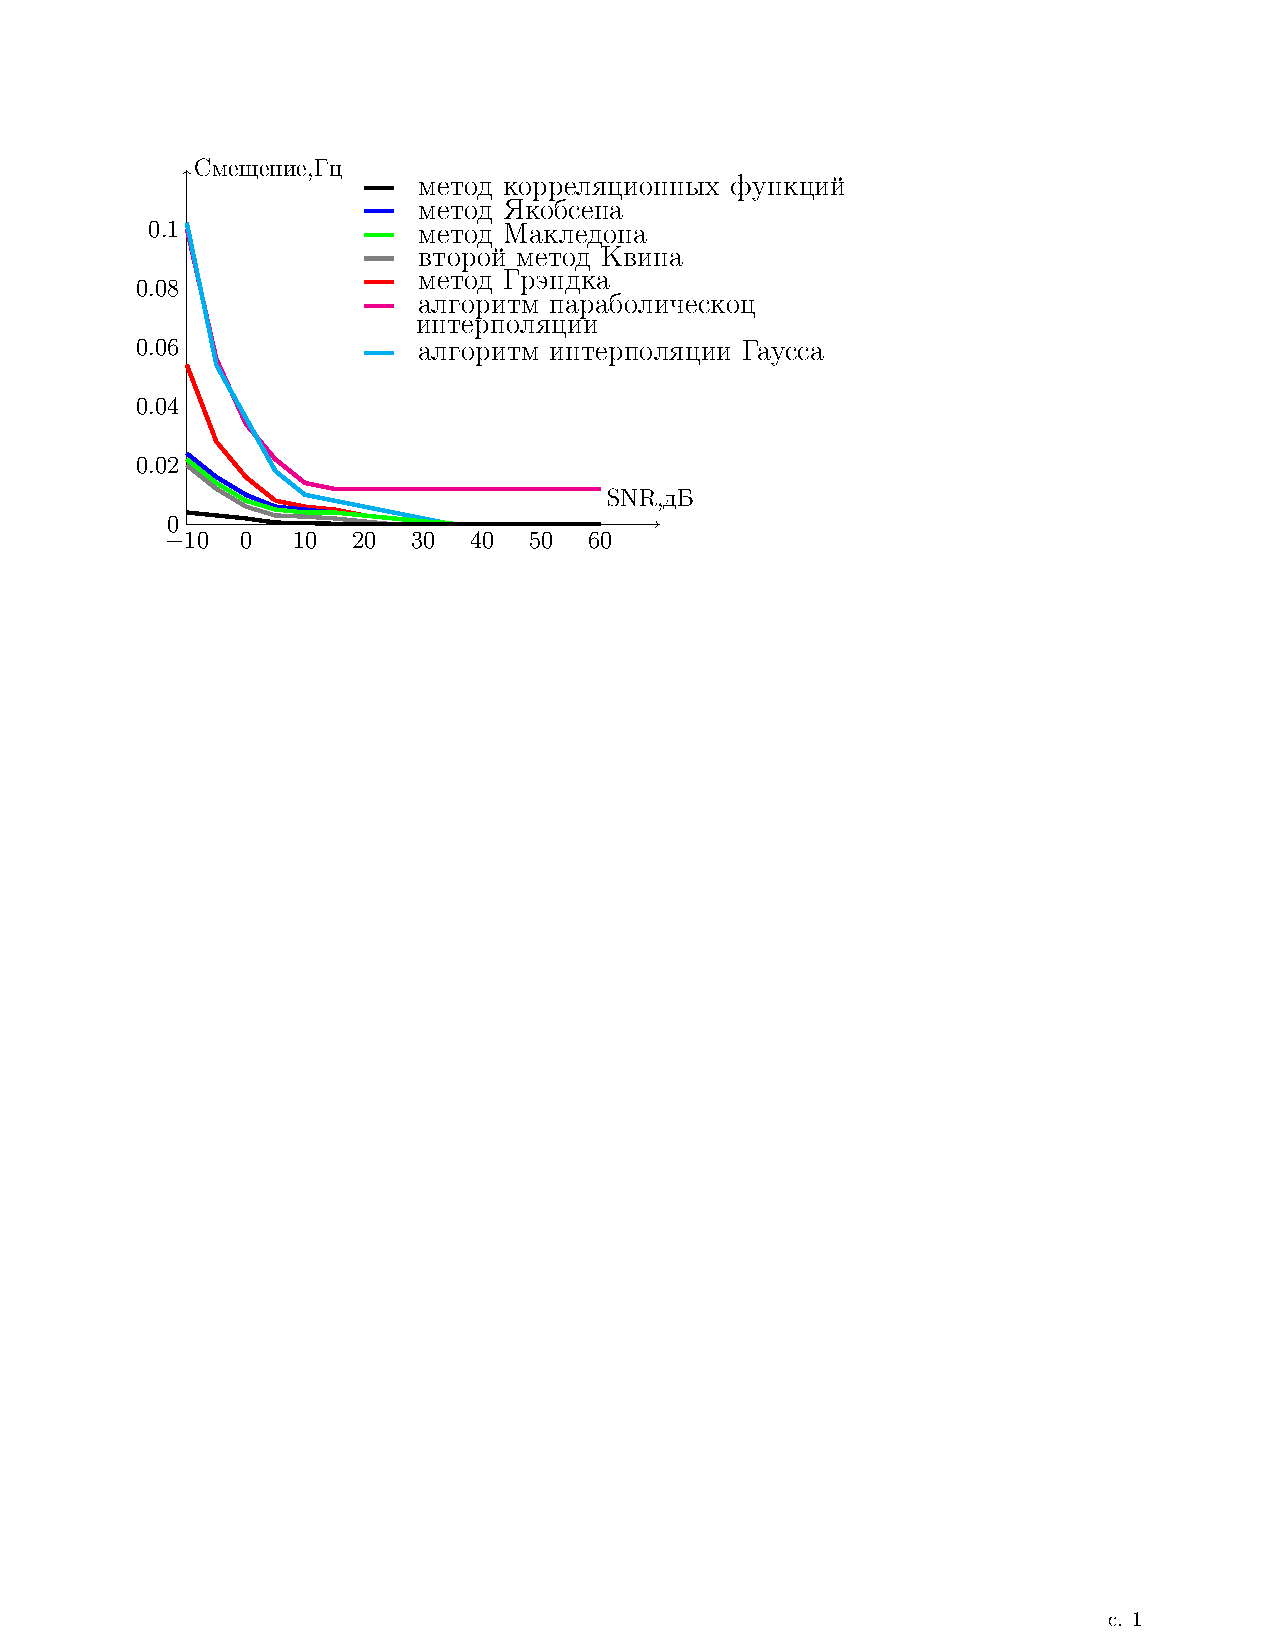
\includegraphics [scale=0.53] {Fundamental frequency offset versus noise level.pdf}
	\caption{Графики зависимостей смещения основной частоты от уровня шума.}
	\label{img:Fundamental_frequency_offset_versus_noise_level}
\end{figure}
&
\begin{figure}[ht]
	\centering
	
\includegraphics [scale=0.43] {Dispersion in the estimation of the fundamental frequency of the voltage.pdf}
	\caption{Дисперсия при оценке основной частоты напряжения.}
	\label{img:Dispersion_in_the_estimation_of_the_fundamental_frequency_of_the_voltage}
\end{figure}
\end{tabular}
\end{frame}

\subsection{Уточнение границы Крамера-Рао}
\begin{frame}{Оценка дисперсии амплитуды гармоники}
	\textsc{Основные результаты из статьи <<Граница Крамера-Рао для амлитуды гармоники при использовании оконных функций>>}:
\begin{itemize}
\item Оценку точности результатов для данных, которые сами по себе являются оценкой точности, выполнить на прямую довольно затруднительно. Во всех трех экспериментах с увеличением числа опытов экспериментальные кривые сглаживались и становились визуально не отличимые от расчетных данных.
\item Эксперименты были проведены при различных входных параметрах (число точек, амплитуда, частота и фаза сигналов, дисперсия шума или коэффициент окна). Ни в одном случае не было зафиксировано отклонение результатов эксперимента от результатов, полученных по предложенной формуле.
\item Таким образом, результаты моделирования алгоритма оценки амплитуды гармоники в условиях шума при наложении оконной функции подтверждают полученные соотношения для оценки дисперсии оценки амплитуды.
\end{itemize}	
\end{frame}

\begin{frame}{Экспериментальная проверка формулы для оценки дисперсии}
\begin{tabular}{m{0.30\linewidth}m{0.32\linewidth}m{0.32\linewidth}}
\begin{figure}[ht]
	\centering
	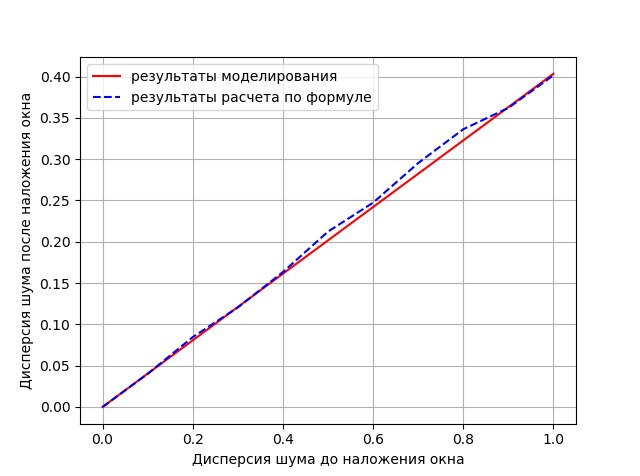
\includegraphics [scale=0.24] {noise_win_var.png}
	\caption{\small{Зависимость дисперсии шума после наложении на него окна.}}
	\label{img:noise_win_var}
\end{figure}
\scriptsize{\begin{equation}
		\label{eq:equation7}
		\sigma^{'2}=\frac{\sum_{n=0}^{N-1} w_n^2}{N}*\sigma^2
\end{equation}}
& 
\begin{figure}[ht]
	\centering
	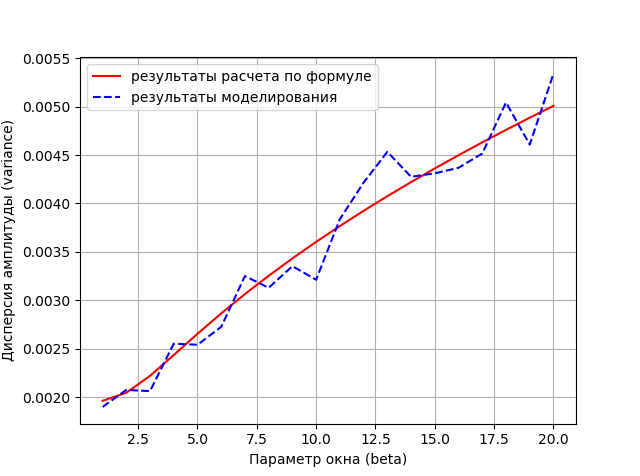
\includegraphics [scale=0.24] {estimate_amp_sin_kaiser_beta.png}
	\caption{\footnotesize{Зависимость дисперсии оценки амплитуды от параметра окна.}}
	\label{img:estimate_amp_sin_kaiser_beta}
\end{figure}
\scriptsize{\begin{equation}
		\label{eq:equation11}
		var(A)\geq \frac{2\sigma^2}{N} \frac{\sum_{n=0}^{N-1}w_n^2}{\left(\sum_{n=0}^{N-1} w_n \right)^2} 			  
\end{equation}}
&
\begin{figure}[ht]
	\centering
	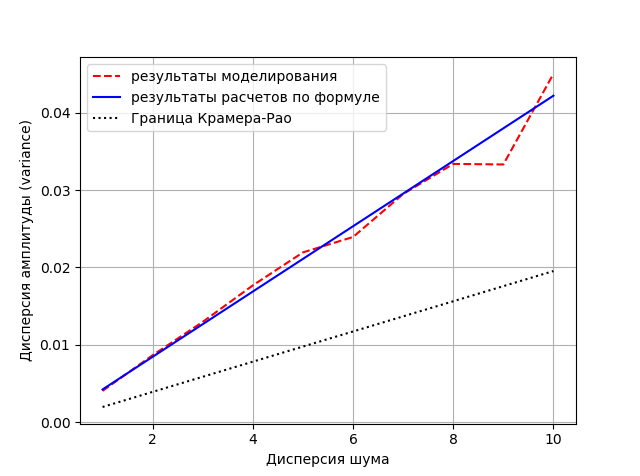
\includegraphics [scale=0.25] {estimate_amp_sin_kaiser_noise.png}
	\caption{\footnotesize{Зависимость дисперсии оценки амплитуды от дисперсии шума.}}
	\label{img:estimate_amp_sin_kaiser_noise}
\end{figure}
\scriptsize{\begin{equation}
		\label{eq:equation11}
		var(A)\geq \frac{2\sigma^2}{N} \frac{\sum_{n=0}^{N-1}w_n^2}{\left(\sum_{n=0}^{N-1} w_n \right)^2} 			  
\end{equation}}
\end{tabular}
\end{frame}

\begin{frame}{Дополненная математическая модель многотонального сигнала}
    \begin{center}
		\Large
		Математическая модель многотонального сигнала для оценки параметров гармоник
	\end{center}	
	\begin{itemize}
		\item Математическое описание свойств ДПФ.
		\item Математическое описание влияния оконных функций.
		\item \textbf{Формулы для оценки дисперсии результатов измерений}.
	\end{itemize}
\end{frame}

\section{Анализ многотональных сигналов}

\subsection{Нахождение гармоники сигнала}
\begin{frame}{Интерполирование спектра}

\scriptsize{
\begin{equation}
	\label{eq:equation3.10}
	A_{\nu} =  \sqrt{\left({\displaystyle\sum_{i=1}^{i=M}\mathrm{Re}(Y_i) \cdot W_{ji}} \right)^2 + \left({\displaystyle\sum_{i=1}^{i=M}\mathrm{Im}(Y_i) \cdot W_{ji}} \right)^2}
\end{equation}
\begin{equation}
	\label{eq:equation3.8.9}
	\varphi = \arctan \left({\frac{\displaystyle\sum_{i=1}^{i=M} \mathrm{Im}(Y_i) \cdot W_{ji}}{\displaystyle\sum_{i=1}^{i=M} \mathrm{Re}(Y_i) \cdot W_{ji}}
	}\right) 
\end{equation}}
\begin{tabular}{m{0.45\linewidth}m{0.45\linewidth}}	
\begin{figure}[ht]
	\centering
	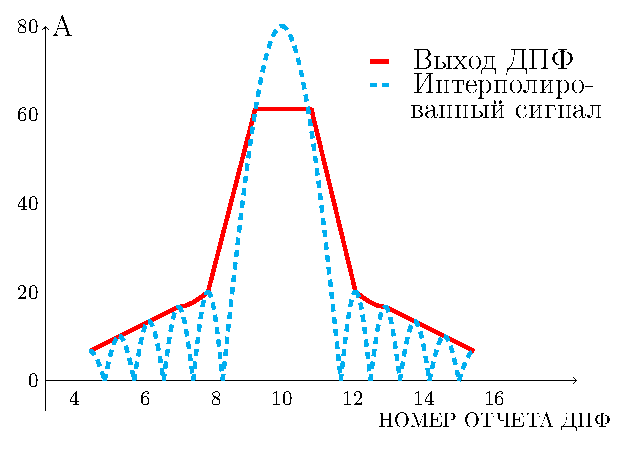
\includegraphics [scale=0.4] {Jacobsen's_method1.pdf}
	\caption{Интерполяция пиков.}
	\label{img:Jacobsen's_method}
\end{figure}
%\textsc{Слева - прямое интерполирование, справа - метод корреляционных функций}
&
\begin{figure}[ht]
	\centering
	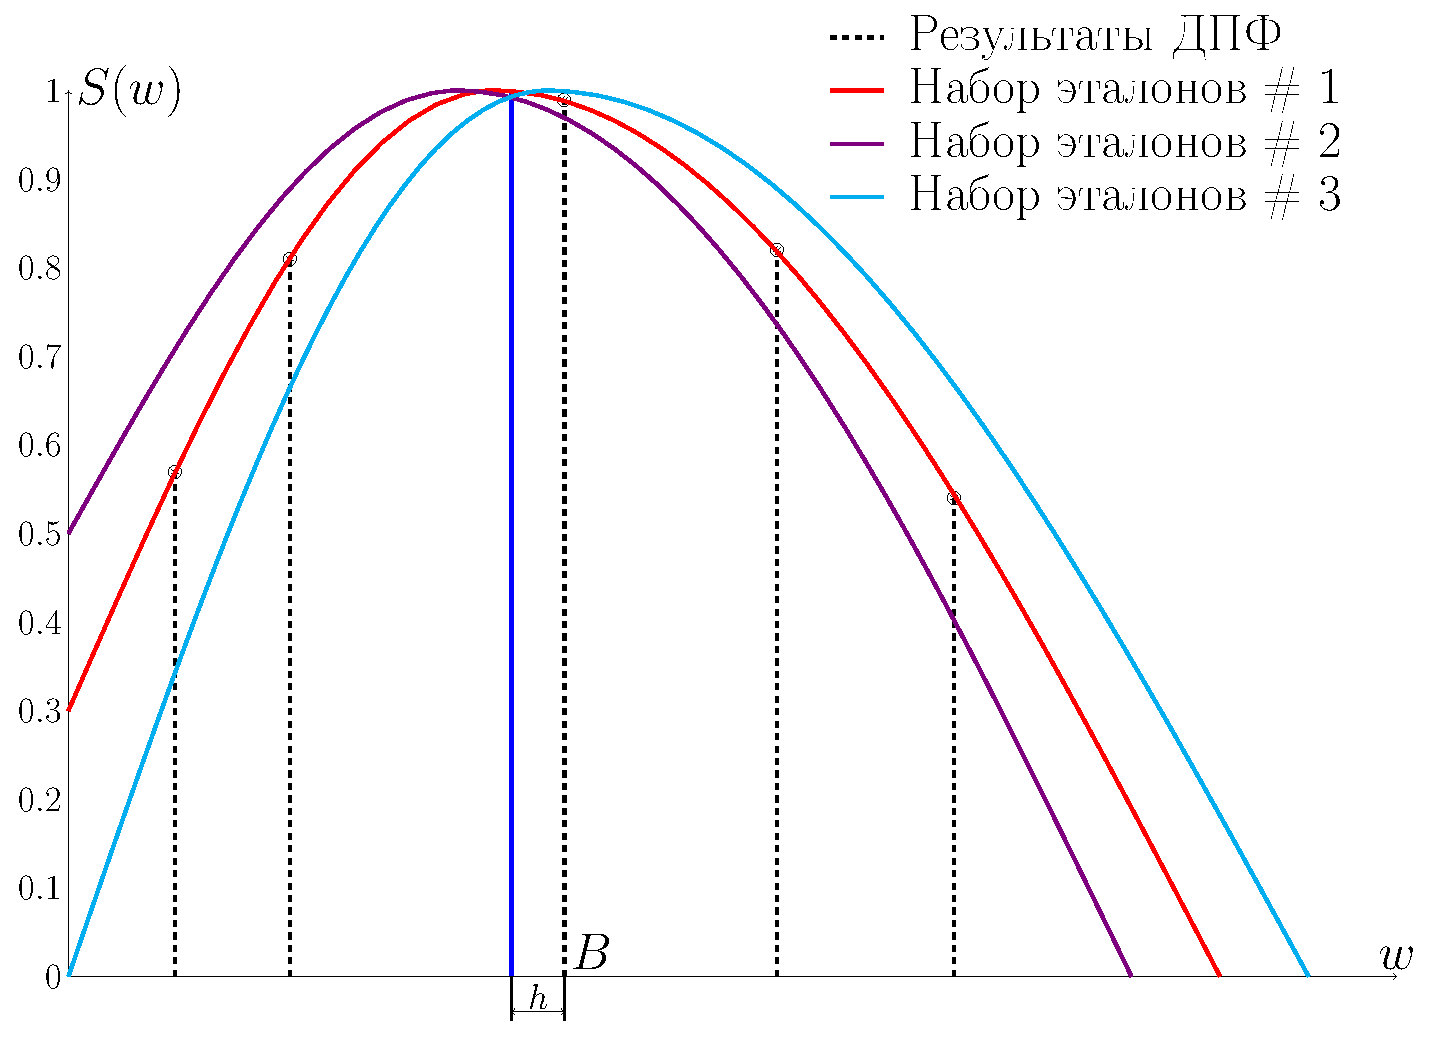
\includegraphics [scale=0.19] {set_of_standards1.pdf}
	\caption{Пример построения наборов эталонов.}
	\label{img:set_of_standards}
\end{figure}	
\end{tabular}
\end{frame}

\begin{frame}{Двойное интерполирование сигнала и спектра}
	\begin{minipage}[t]{0.43\linewidth}
		\centering 
		\textbf{Сигнал (частота=5.2)}
		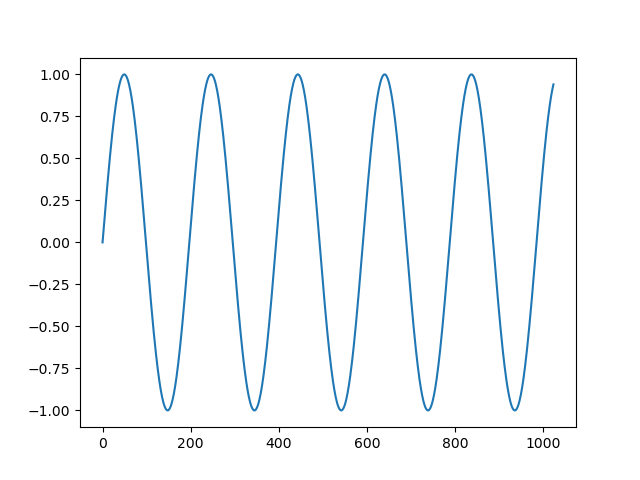
\includegraphics[width=.85\linewidth]{signal}
		\textbf{Экстраполированный \\ сигнал ($k_{i1}=4$)}
		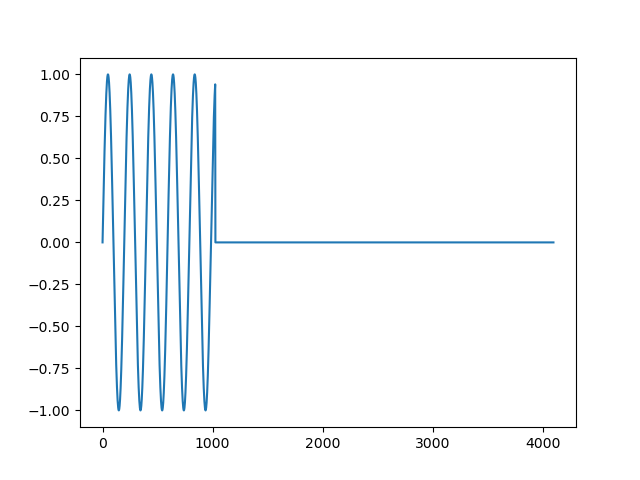
\includegraphics[width=.85\linewidth]{interpolated_signal}		
	\end{minipage}
	\hfill
	\begin{minipage}[t]{0.43\linewidth}
		\centering 
		\textbf{Спектр сигнала}
		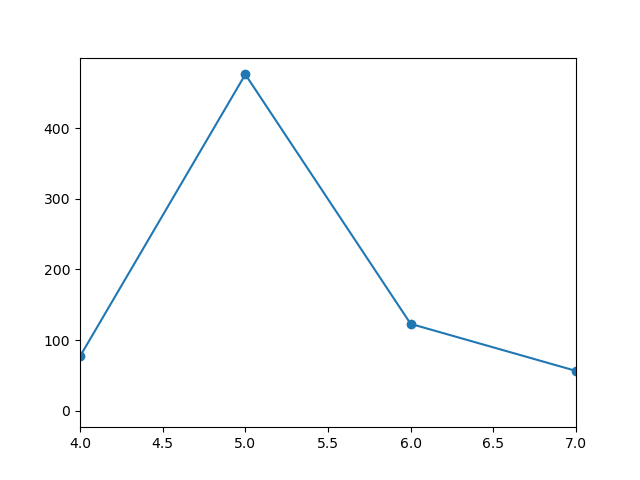
\includegraphics[width=.85\linewidth]{spectrum_double}
		\textbf{Спектр с двойной интерполяцией ($k_{i2}=4$)}
		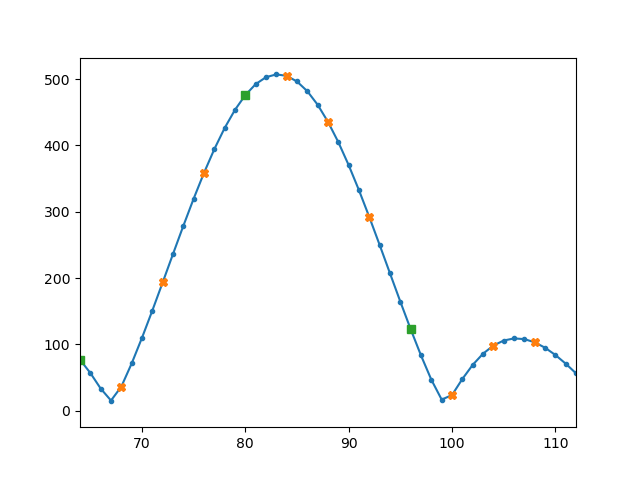
\includegraphics[width=.85\linewidth]{spectrum_double_interpolated}
	\end{minipage}
\end{frame}

\subsection{Поиск гармоник}
\begin{frame}{Алгоритм поиска гармоник}
%	\textsc{ГСА алгоритма поиска гармоник из зарегистрированной программы}
\begin{figure}[ht]
	\centering
	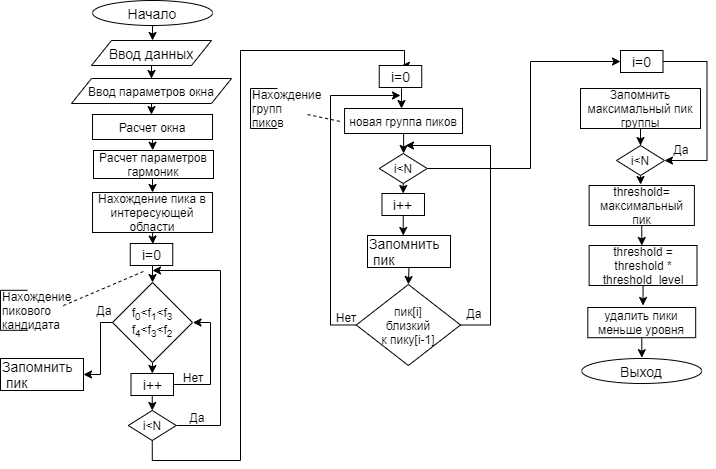
\includegraphics [scale=0.40] {Diagram_GSA2.png}
	\caption{ГСА алгоритма поиска гармоник.}
	\label{img:Diagram_GSA}
\end{figure}
\end{frame}

\begin{frame}{Расчет гармоник и интергармоник}
	\textsc{Свидетельство о регистрации программы}
\begin{tabular}{m{0.45\linewidth}m{0.45\linewidth}}
\begin{figure}[ht]
	\centering
	
\includegraphics [scale=0.07] {Computer_program1.jpg}
	\caption{Свидетельство.}
	\label{img:Computer_program}
\end{figure}
&
\begin{figure}[ht]
	\centering
	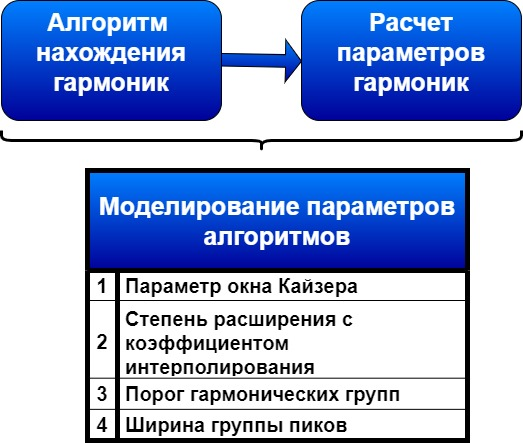
\includegraphics [scale=0.3] {Diagram_Computer_program2.jpg}
	\caption{Функционал в зарегистрированной программе.}
	\label{img:Diagram_Computer_program}
\end{figure}
%Предлагаемая полезная модель относится к электроизмерительной технике и может быть использована для определения гармоник.
\end{tabular}
\end{frame}

\subsection{Практическая реализация}
\begin{frame}{Метод нахождения параметров гармоник}
	\begin{block}{При заданной точности по частоте}
		$k_i=\frac{f_1}{f_{eps}}$, 
		
		${f_{eps}}$ -- заданная точность
	\end{block}	
	\begin{block}{При заданной точности по амплитуде}
		$f_{eps}=a_{eps}*\frac{sw_0-w_1}{sw_0}$,  
		
		$a_{eps}$ -- заданная точность, $sw_i$ -- отсчеты спектра окна.
	\end{block}
	\begin{block}{При заданном шуме}
		$a_{eps} = var(A)\geq \frac{2\sigma^2}{N} \frac{\sum_{n=0}^{N-1}w_n^2}{\left(\sum_{n=0}^{N-1} w_n \right)^2}$ Формула для оценки дисперсии амплитуды
	\end{block}
\end{frame}


\begin{frame}{Использование корреляции}
\begin{tabular}{m{0.45\linewidth}m{0.49\linewidth}}
	\begin{figure}[ht]
		\centering
		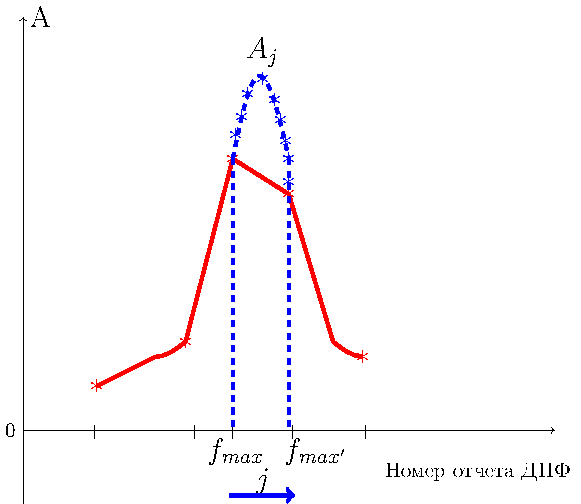
\includegraphics [scale=0.5] {Using_correlation.pdf}
		\caption{Использование корреляции.}
		\label{img:Using_correlation}
	\end{figure}
&
\begin{equation}
\label{eq:equation3.10}
j = 0, 1, \cdots M-1
\end{equation}
\begin{equation}
\label{eq:equation3.10}
f_j = \frac{\left| f_{max}- f_{max'} \right| }{M} + f_{max'}
\end{equation}
\begin{equation}
\label{eq:equation3.10}
A_j = 
\displaystyle\sum_{k=0}^{M-1} x(k) \cdot \exp \left( -f_j \cdot \frac{2 \pi k}{N}\right) 
\end{equation}

$f_{max}$ -- частота гармоники ДПФ с наибольшей амплитудой.

$f_{max}'$ -- частота гармоники ДПФ со 2 по величине амплитуде.
\end{tabular}
\end{frame}

\begin{frame}{Pruned FFT}
\begin{tabular}{m{0.45\linewidth}m{0.49\linewidth}}
\begin{figure}[ht]
	\centering
	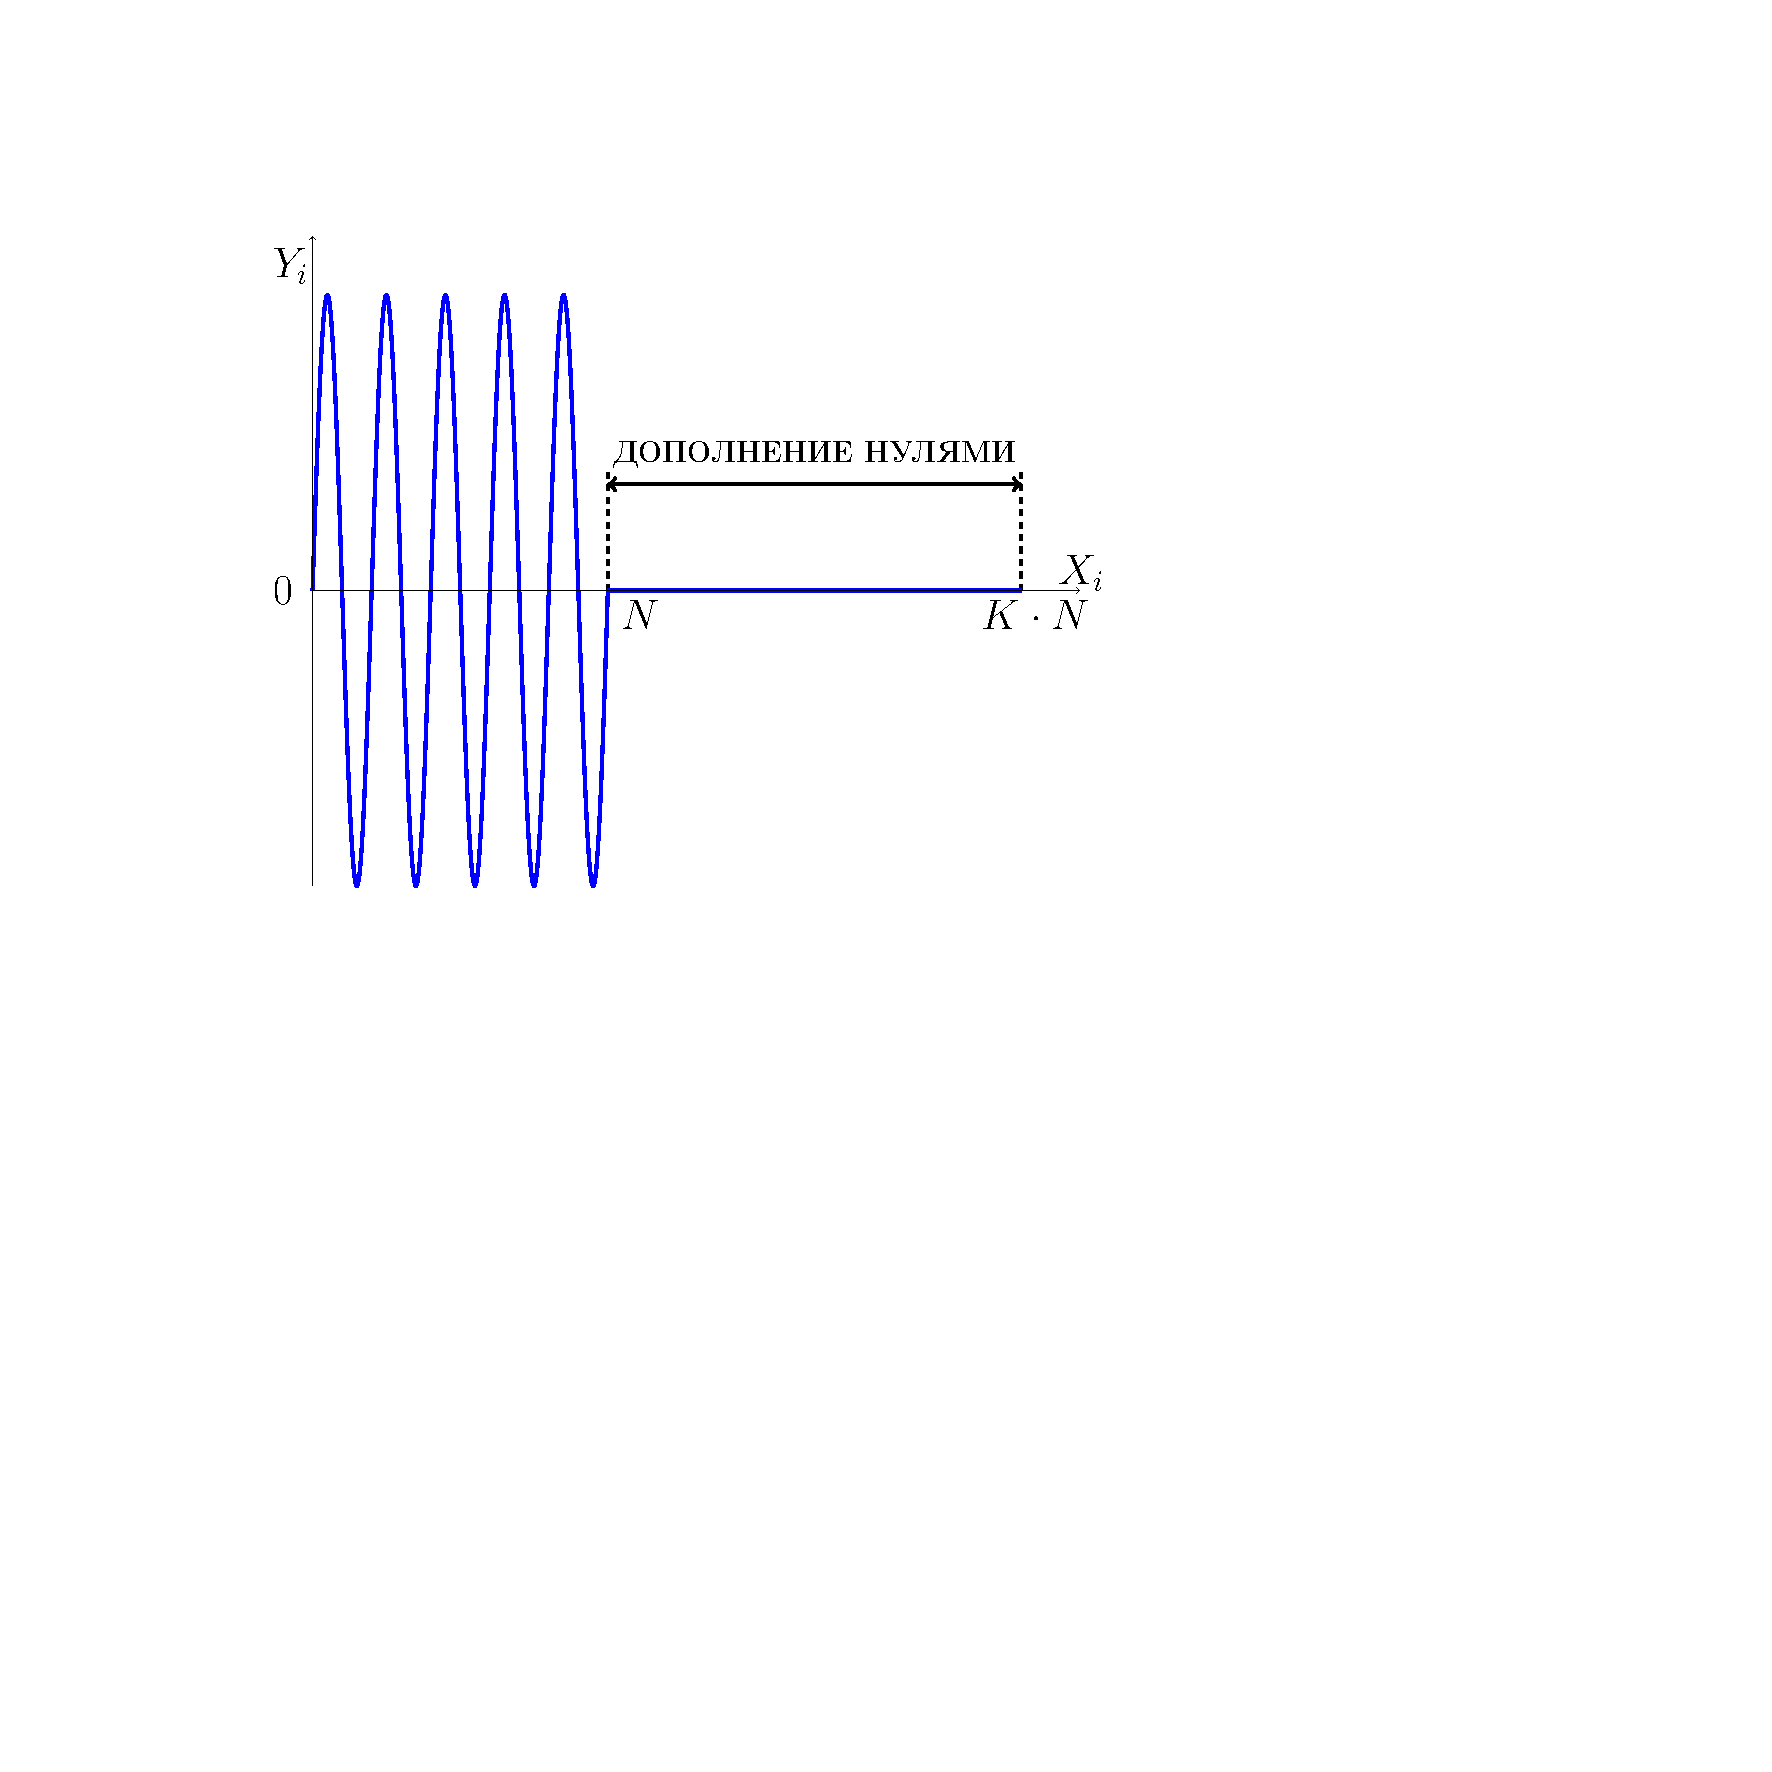
\includegraphics [scale=0.3] {Pruned_FFT.pdf}
	\caption{Исходный сигнал.}
	\label{img:Pruned_FFT}
\end{figure}
\textbf{Матричная форма:}
\tiny{
\begin{center}
	$\longrightarrow N$	
\end{center}
\begin{equation}
\label{eq:equation111}
\downarrow K 
	\begin{pmatrix}
	X_{0} & X_{1} & \cdots & X_{n-1} \\
	X_{N} & X_{n+1} & \cdots & X_{2n-1} \\
	\vdots  & \vdots  & \ddots & \vdots  \\
	X_{N(k-1)} & \cdots & \cdots & X_{N(k-1)} 
	\end{pmatrix}
\Bigg \} {\text{НУЛИ}}
\end{equation}} 
&
\textbf{Обобщаем алгоритм Кули-Тьюки:}
\begin{enumerate}
	\item Вычисляем БПФ столбцов;
	\item Умножаем на поворачивающие множители;
	\item Вычисляем БПФ строк.
\end{enumerate}
\textbf{Pruned FFT}
\begin{itemize}
	\item Не требует $1$-й стадии вычислений;
	\item Сложность алгоритма $N \cdot \log(N) \cdot K$;
	\item Сложность растет линейно с ростом $K$.
\end{itemize}
\end{tabular}
\end{frame}

%\begin{frame}{Анализ быстродействия}
%	\begin{block}{}
%		\begin{minipage}[t]{0.47\linewidth}
%			\centering \textcolor{blue}{\textbf{Прямой метод}}
%			%\textsc{Найти график, желательно с CUDA}	
%			\begin{figure}[ht]
%				\centering
%				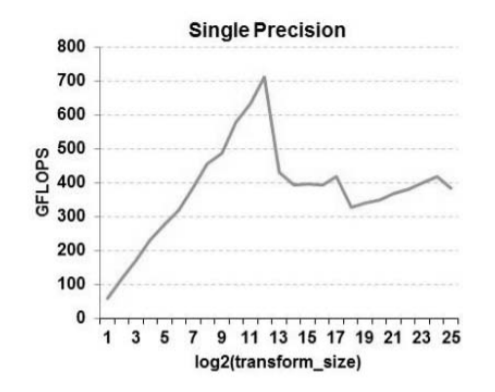
\includegraphics [scale=0.27] {CUDA.PNG}
%				%\caption{CUDA.}
%				\label{img:CUDA}
%			\end{figure}			
%			%\textcolor{blue}{\textit{Не подходит для встроенных систем}}
%		\end{minipage}
%		\begin{minipage}[t]{0.47\linewidth}
%			\centering \textcolor{blue}{\textbf{Sparse FFT}}
%			%\textsc{График с сайта}		
%			\begin{figure}[ht]
%				\centering
%				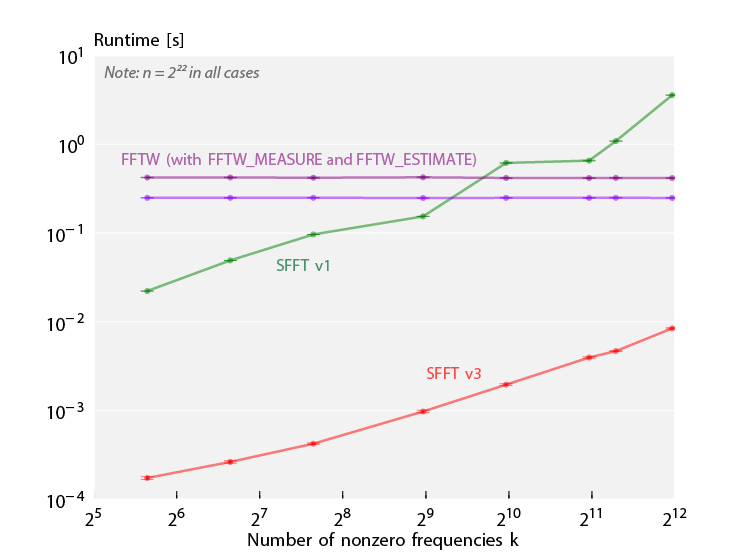
\includegraphics [scale=0.25] {Sparse_Fourier_Transform_Performance.png}
%				%\caption{Sparse FFT.}
%				\label{img:Sparse_Fourier_Transform_Performance}
%			\end{figure}
%			%\textcolor{blue}{\textit{Не работает с интерполированными сигналами}}
%		\end{minipage}
%	\end{block}
%	\hfil
%	\begin{block}{}
%		\begin{minipage}[t]{0.47\linewidth}
%			\centering \textcolor{blue}{\textbf{Быстрая корреляция}}
%			%\textsc{Найти график}	
%			\begin{figure}[ht]
%				\centering
%				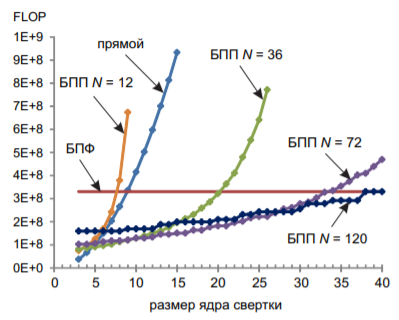
\includegraphics [scale=0.3] {Прямая_корреляция2.PNG}
%				%\caption{Быстрая корреляция.}
%				\label{img:Прямая_корреляция}
%			\end{figure}			
%			%\textcolor{blue}{\textit{Высокое быстродействие при малом коэффициенте интерполирования}}	
%		\end{minipage}
%		\begin{minipage}[t]{0.47\linewidth}
%			\centering \textcolor{blue}{\textbf{Pruned БПФ}}
%			%\textsc{Найти график}	
%			\begin{figure}[ht]
%				\centering
%				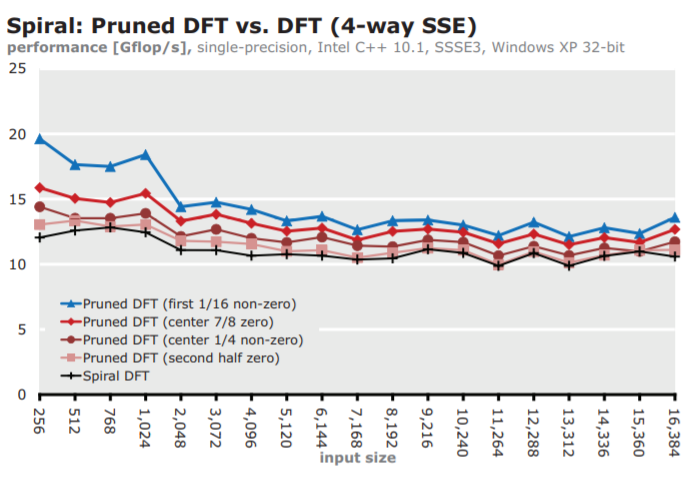
\includegraphics [scale=0.25] {Pruned_DFT.PNG}
%				%\caption{Pruned БПФ.}
%				\label{img:Pruned_DFT}
%			\end{figure}			
%			%\textcolor{blue}{\textit{Относительно высокое быстродействие, слабо зависит от коэффициента интерполирования}}	
%		\end{minipage}
%	\end{block}
%\end{frame}

\begin{frame}{Анализ быстродействия}
	\begin{minipage}[t]{0.45\linewidth}
	\centering 
	\textbf{Быстрая корреляция}
	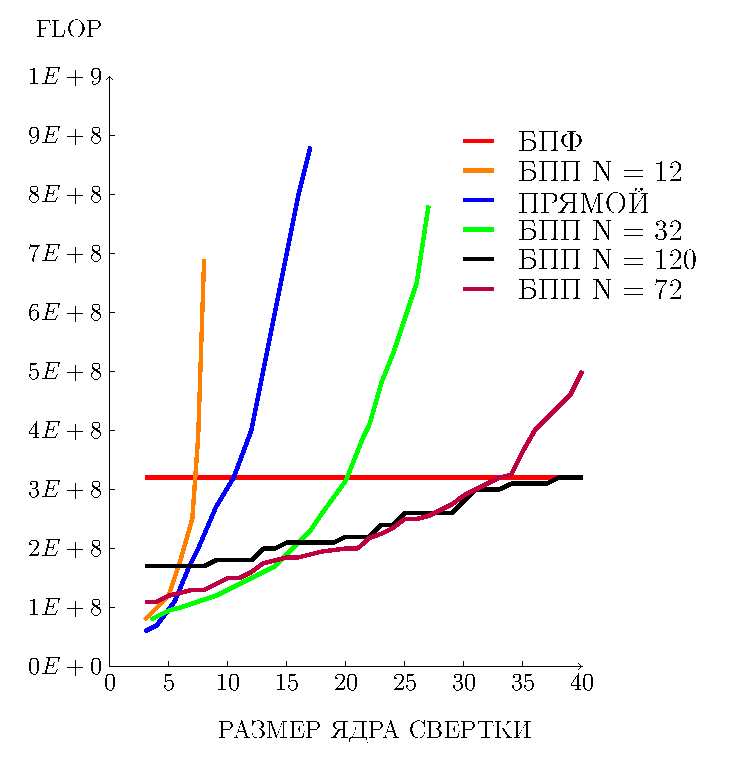
\includegraphics[width=.745\linewidth]{Direct correlation.pdf}
	\textbf{Pruned БПФ}
	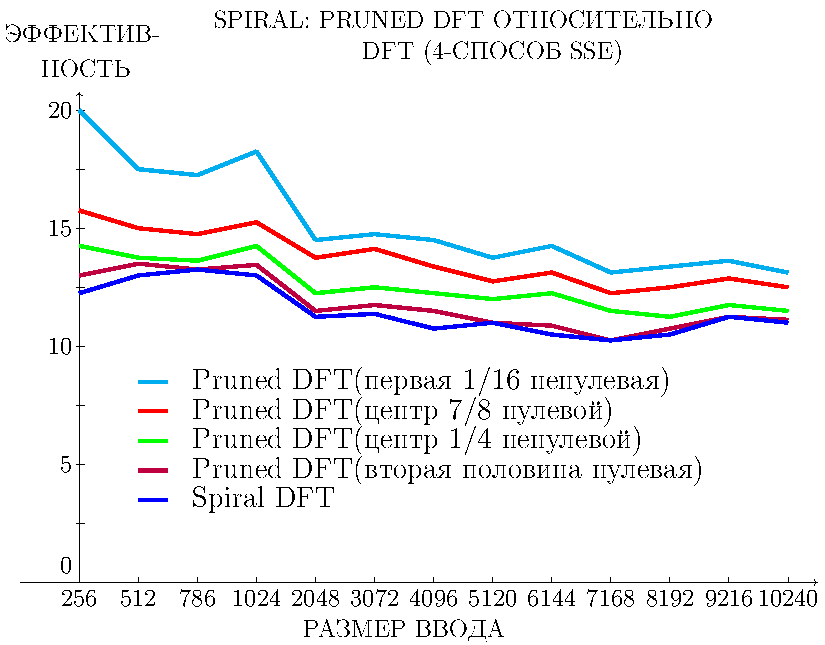
\includegraphics[width=.745\linewidth]{Pruned DFT2.pdf}		
\end{minipage}
\hfill
\begin{minipage}[t]{0.45\linewidth}
	\centering 
	\textbf{Прямой метод}
	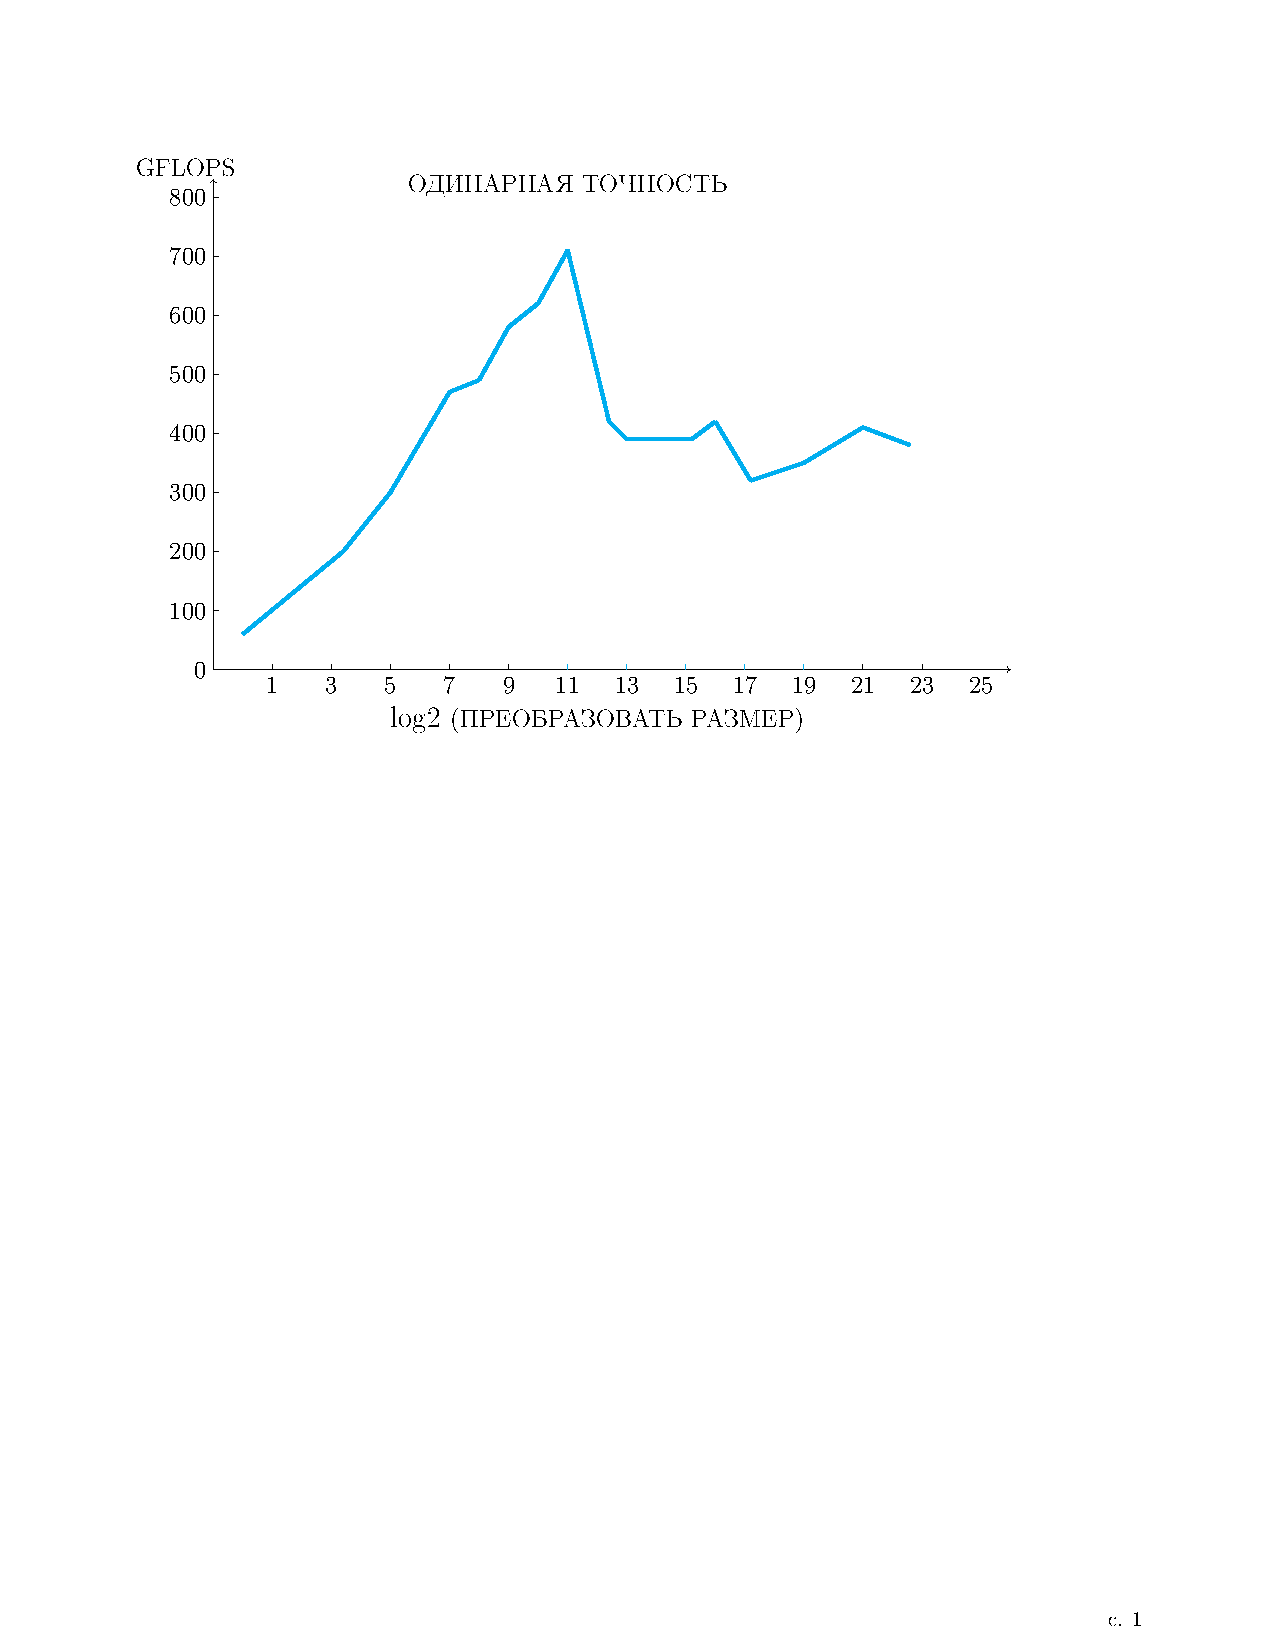
\includegraphics[width=.9\linewidth]{CUDA.pdf}
	\textbf{Sparse FFT}
	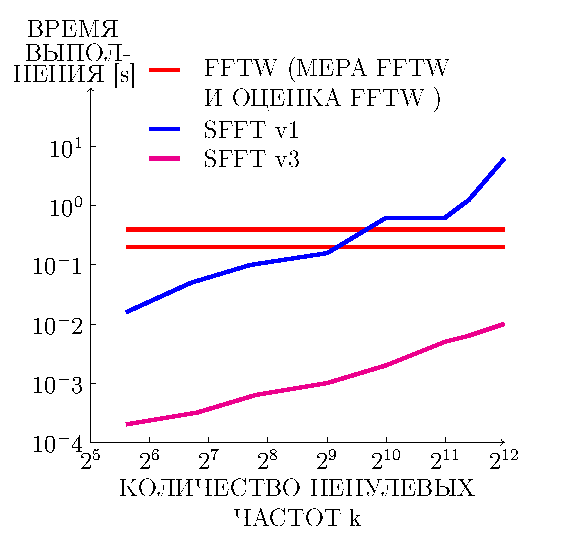
\includegraphics[width=.8\linewidth]{Sparse Fourier Transform2.pdf}
\end{minipage}
\end{frame}



\section{Заключение}

\subsection{Результаты работы}
\begin{frame}{Список опубликованных работ}
\scriptsize{
\textbf{В изданиях из перечня ВАК Минобрнауки России:}	
\begin{itemize}
	\item Альтман Е.~А., Захаренко Е.~И., Васеева Т.~В. Применение метода разложения двумерной свертки при реализации цифровых фильтров // Научный вестник Новосибирского государственного технического университета. – $2017$. – \textnumero.~$4$. – С. $95$-$104$.
	
	\item Лаврухин А.~А., Малютин А.~Г., Васеева Т.~В. Повышение эффективности информационно-измерительного комплекса автоматизированной системы мониторинга и учета электроэнергии // Известия Транссиба. – $2018$. – \textnumero.~$4 (36)$.
\end{itemize}}	
\scriptsize{
\textbf{SCOPUS:}	
\begin{itemize}
	\item Altman E.~A., Vaseeva T.~V., Aleksandrov A.~V. Cache-aware algorithm for multidimensional correlations //Journal of Physics: Conference Series. – IOP Publishing, $2019$. – Т. $1260$. – \textnumero.~$4$. – С. $042001$.
\end{itemize}}

\scriptsize{
\textbf{В прочих изданиях:}
\begin{itemize}
	\item Васеева, Т.~В. Граница Крамера-Рао амплитуды однотонального сигнала для методов ее оценки с использованием оконных функций / Т.~В. Васеева, Е.~А. Альтман //Инновационные проекты и технологии в образовании, промышленности и на транспорте. – $2021$. – С. $301$-$307$.
	
	\item Васеева Т.~В., Альтман Е.~А., Александров А.~В. Cравнительное исследование гармонических и интергармонических методов оценки сигналов //Инновационные проекты и технологии в образовании, промышленности и на транспорте. – $2020$. – С. $51$-$57$.
		
	\item Малютин А.~Г. и др. Математическое моделирование и численные методы для исследования алгоритмов обработки сигналов и анализа систем массового обслуживания. – $2020$.
\end{itemize}}
\end{frame}	

\begin{frame}{Результаты работы}
\scriptsize{
\begin{itemize}
	\item Альтман Е.~А., Васеева Т.~В., Александров А.~В. Граница Крамера-Рао для амплитуды гармоники при использовании оконных функций // Динамика систем, механизмов и машин. – $2020$. – Т. $8$. – \textnumero.~$2$. – С. $145$-$152$.
	
	\item Малютин А.~Г. и др. Математическое моделирование, численные методы и комплексы программ для решения задач обработки сигналов и измерения характеристик технических систем. – $2019$.
	
	\item  Малютин А.~Г. и др. Совершенствование подходов, архитектур и алгоритмов информационно-управляющих систем и средств измерения. – $2019$.
		
	\item Альтман Е.~А., Васеева Т.~В., Александров А. В. Оценка сложности алгоритма БПФ при моделировании его работы // Инновации в информационных технологиях, машиностроении и автотранспорте. – $2019$. – С. $116$-$118$.
	
	\item Альтман Е.~А., Александров А.~В., Васеева Т.~В. Современные информационные технологии разработки программ для обработки радиотехнических сигналов на примере БПФ // Надежность функционирования и информационная безопасность инфокоммуникационных, телекоммуникационных и радиотехнических сетей и систем. – $2019$. – С. $132$-$139$.
	
	\item Васеева Т.~В., Альтман Е.~А., Елизаров Д.~А. Сравнительный анализ методов определения параметров гармоник сигнала электрической сети // Инновационные проекты и технологии в образовании, промышленности и на транспорте. – $2019$. – С. $261$-$267$.

	\item Васеева Т.~В., Альтман Е.~А., Александров А.~В. Сравнительный анализ применения алгоритмов определения частоты при оценке гармоник в электрических сетях // Системы управления, информационные технологии и математическое моделирование. – $2019$. – С. $61$-$66$.
\end{itemize}}
\end{frame}

\begin{frame}{Результаты работы}
\scriptsize{
\begin{itemize}
	\item Альтман Е.~А., Васеева Т.~В., Александров А.~В. Кэш-ориентированный алгоритм для вычисления многомерной корреляции // Проблемы машиноведения. – $2019$. – С. $385$-$389$.
	
	\item Малютин А. Г. и др. Математическое моделирование, численные методы и комплексы программ для решения задач обработки сигналов и анализа структуры информационной системы. – 2018.
	
	\item Васеева Т.~В., Альтман Е.~А., Малютин А.~Г. Применение быстрых алгоритмов для выполнения фильтрации изображений // Современные проблемы радиоэлектроники. – $2018$. – С. $162$-$165$.
	
	\item Альтман Е.~А., Афанасьева Н.~С., Васеева Т.~В. Расширение глубины резкости изображений программным способом // Инновационные проекты и технологии в образовании, промышленности и на транспорте. – $2018$. – С. $222$-$227$.
	
	\item Васеева Т.~В., Альтман Е.~А. Исследование точности математических моделей алгоритмов реализованных на языках высокого уровня // Информационные и управляющие системы на транспорте и в. – $2018$. – С. $236$.
	
	\item Александров А.~А., Васеева Т.~В., Ананьева Н.~Г. Оценка эффективности алгоритма корреляции для различных аппаратных платформ // Тезисы $XIX$ Всероссийской конференции молодых учёных по математическому моделированию и информационным технологиям. – $2018$. – С. $54$-$54$.
	
	\item Васеева Т.~В., Альтман Е.~А., Елизаров Д.~А. Информационно-измерительная система для анализа гармоник сигнала в электрической сети // САПР и моделирование в современной электронике. – $2018$. – С. $131$-$135$.	
\end{itemize}}
\end{frame}

\begin{frame}{Результаты работы}
\scriptsize{
\begin{itemize}
	\item Васеева Т.~В., Александров А.~В. Реализация алгоритмов вычисления корреляции для диагностирования подвижного состава методами корреляционного анализа // Технологическое обеспечение ремонта и повышение динамических качеств железнодорожного подвижного состава. – $2017$. – С. $138$-$142$.
	
	\item Терентьева А.~В., Васеева Т.~В., Кильдибеков А.~Б. Алгоритм детектирования лиц в различных ракурсах и наклонах // Инновационные проекты и технологии в образовании, промышленности и на транспорте. – $2017$. – С. $250$-$255$.
	
	\item Васеева Т.~В., Альтман Е.~А. Распознавание границ движущихся объектов методами компьютерного зрения // Информационно-телекоммуникационные системы и технологии. – $2017$. – С. $304$-$306$.
	
	\item Альтман Е.~А., Васеева Т.~В., Кузнецов Д.~И. Моделирование алгоритмов обработки сигналов с целью оптимизации их аппаратной реализации // Современные научные исследования и разработки. – $2017$. – \textnumero.~$4$. – С. $27$-$29$.	
	
	\item Альтман Е.~А., Дикаревич Н.~С., Васеева Т.~В. Детекторы локальных особенностей в системах компьютерного зрения, применяемых на железнодорожном транспорте // Инновационные проекты и технологии в образовании, промышленности и на транспорте. – $2016$. – С. $272$-$280$.
\end{itemize}}
\end{frame}

\subsection{Основные положения, выносимые на защиту}
\begin{frame}{Основные положения выносимые на защиту}
	\begin{enumerate}
		\item Дополнение к математической модели многотонального сигнала в виде формулы, позволяющей определить дисперсию оценки амплитуды гармоники, отличающемуся от известной границы Крамера-Рао учетом изменения дисперсии после применения оконных функций.
		\item Основанный на корреляционном анализе численный метод, позволяющий определить параметры гармоник сигналов с точностью, определяемой уточненной границей Крамера-Рао, включающий в себя вычислительно-эффективную схему расчета корреляций и отличающийся от известных методов отсутствием потерь в точности результатов при интерполировании параметров гармоник.
		\item Комплекс программ для анализа и построения алгоритмов оценки параметров многотональных сигналов.
	\end{enumerate}
\end{frame}

       % Настройки заглавной странице
\chapter*{Заключение}                       % Заголовок
\addcontentsline{toc}{chapter}{Заключение}  % Добавляем его в оглавление

%% Согласно ГОСТ Р 7.0.11-2011:
%% 5.3.3 В заключении диссертации излагают итоги выполненного исследования, рекомендации, перспективы дальнейшей разработки темы.
%% 9.2.3 В заключении автореферата диссертации излагают итоги данного исследования, рекомендации и перспективы дальнейшей разработки темы.
%% Поэтому имеет смысл сделать эту часть общей и загрузить из одного файла в автореферат и в диссертацию:

Основные результаты работы заключаются в следующем.
%%% Согласно ГОСТ Р 7.0.11-2011:
%% 5.3.3 В заключении диссертации излагают итоги выполненного исследования, рекомендации, перспективы дальнейшей разработки темы.
%% 9.2.3 В заключении автореферата диссертации излагают итоги данного исследования, рекомендации и перспективы дальнейшей разработки темы.
В результате проведенных исследований получены новые научные результаты и технические решения и разработки, направленные на повышение достоверности, точности и эффективности работы алгоритмов оценивания параметров гармоник.

Их применение позволит обеспечить высокое качество разработки контрольно-измерительных приборов для электрических сетей, а также может быть использованы при создании устройств приема информации для радиосигналов и других систем обработки сигналов.

Основные научные и практические результаты диссертационной работы состоят в следующем:
\begin{enumerate}
  \item Произвели обзор методов: интерпорилрование спектра (метод Якобсена, два метода Квина, два метода Маклеода, метод Грэндка, алгоритм параболической интерполяции, алгоритм интерполяции Гаусса), алгоритм, рекомендованный в ГОСТ $30804.4.7-2013$, метод корреляционныход  функций, Модернизированный метод корреляционных функций, алгоритм вычисления одномерной корреляции, алгоритм вычисления двумерной корреляции, алгоритм дискретного преобразования Фурье (ДПФ), алгоритма быстрого преобразования Фурье (БПФ), алгоритм разряженного преобразования Фурье (Spare FFT). 
  \item Выведена формула для нахождения границы Крамера-Рао при применении оконной функции, которая позволяет повысить эффективность научных исследований различных алгоритмов обработки сигналов с применением оконных функций, заменив моделирование алгоритма с применением различных окон расчетом по предложенной формуле.
  \item Предложенный численный метод, вместе с его быстрой реализацией, позволяют повысить точность и достоверность результатов измерительных приборов для электрических сетей. Численный метод позволяет находить оптимальную несмещенную оценку параметров гармоник.
  \item Разработанный комплекс программ позволяет проводить научные исследования в области цифровой обработки сигналов и используется в учебном процессе: программа прямого корреляционного метода с использование быстрых алгоритмов обработки сигналов, оценка дисперсии белого шума после наложения на него окна, оценка амплитуды при использовании различных окон, оценка амплитуды при различныз уровнях шума, алгоритм вычисления одномерной свертки.
\end{enumerate}

В качестве рекомендаций дальнейшей разработки темы диссертации в части построения математических моделей систем приема и измерения сигналов предлагается распространить подход к определению границы Крамера-Рао для других алгоритмов цифровой обработки сигналов. Перспективным также является изучение и применение разработанных численных методов для оценки гармонических сигналов другого типа, отличного от сигналов в электрической сети.

%И какая-нибудь заключающая фраза.

В заключение автор
выражает благодарность и большую признательность научному руководителю
Альтману~Е.\:А. за поддержку, помощь, обсуждение результатов и~научное
руководство. Также автор благодарит заведующего кафедрой <<Автоматика и системы управления>> Малютина~А.\:Г. и старшего преподавателя Александрова~А.\:В.

    % Последние слайды презентации
\appendix
%\begin{frame}
%    \frametitle{Ответы на замечания ведущей организации НИИ~<<Рога~и~копыта>>}
%    \begin{itemize}
%        \item Замечание -- ответ
%        \item Замечание -- ответ
%        \item Замечание -- ответ
%        \item Замечание -- ответ
%        \item Замечание -- ответ
%    \end{itemize}
%\end{frame}
%
%\begin{frame}
%    \frametitle{Ответы на замечания оф. оппонента Иванова\,И.\,И}
%    \begin{itemize}
%        \item Замечание -- ответ
%        \item Замечание -- ответ
%        \item Замечание -- ответ
%        \item Замечание -- ответ
%        \item Замечание -- ответ
%    \end{itemize}
%\end{frame}
%
%\begin{frame}
%    \frametitle{Ответы на замечания Петрова\,П.\,П}
%    \begin{itemize}
%        \item Замечание -- ответ
%        \item Замечание -- ответ
%        \item Замечание -- ответ
%        \item Замечание -- ответ
%        \item Замечание -- ответ
%    \end{itemize}
%\end{frame}
      % Запасные слайды презентации
\end{document}
